% Seminar 15: Review and exam preparation
% Time Series Analysis -- Bachelor's programmes Economic Informatics and Economic Cybernetics, Bucharest University of Economic Studies
% GENERATED by latex/build_seminar15.py -- edit the generator, not this file.
% Student version by default; the instructor version is the *_solutions.tex wrapper.
\makeatletter\@ifundefined{ifsolutions}{\expandafter\newif\csname ifsolutions\endcsname}{}\makeatother

\newcommand{\coursename}{Time Series Analysis}
% Preambul comun TSA -- Serii de timp / Time Series Analysis (Beamer, 16:9)
% Același design ca MFM și SFM (preluat din SFM, 5 octombrie 2026). Înainte de % Preambul comun TSA -- Serii de timp / Time Series Analysis (Beamer, 16:9)
% Același design ca MFM și SFM (preluat din SFM, 5 octombrie 2026). Înainte de % Preambul comun TSA -- Serii de timp / Time Series Analysis (Beamer, 16:9)
% Același design ca MFM și SFM (preluat din SFM, 5 octombrie 2026). Înainte de \input{../../latex/preamble} se definește
%   \newcommand{\coursename}{Time Series Analysis}      (EN)
%   \newcommand{\coursename}{Serii de timp}       (RO)  și  \def\tsalang{ro}
% Fișierele .tex se află în EN/Courses, EN/Seminars, RO/Cursuri, RO/Seminarii (două niveluri sub rădăcină).
% Deck-urile sînt generate de latex/build_chapterN.py / build_seminarN.py (vezi latex/tsa_build.py).

\documentclass[9pt, aspectratio=169, t]{beamer}
\providecommand{\coursename}{Time Series Analysis}

% Ensure content fits on slides
\setbeamersize{text margin left=8mm, text margin right=8mm}
% Smaller institute font (title page)
\setbeamerfont{institute}{size=\footnotesize}

%=============================================================================
% THEME AND STYLE CONFIGURATION
%=============================================================================
\usetheme{default}
% Using default theme for clean header/footer control

% Color Palette (matching Redispatch PDF)
\definecolor{MainBlue}{RGB}{26, 58, 110}
\definecolor{AccentBlue}{RGB}{26, 58, 110}
\definecolor{IDAred}{RGB}{205, 0, 0}
\definecolor{DarkGray}{RGB}{51, 51, 51}
\definecolor{MediumGray}{RGB}{128, 128, 128}
\definecolor{LightGray}{RGB}{248, 248, 248}
\definecolor{VeryLightGray}{RGB}{235, 235, 235}
\definecolor{KeynoteGray}{RGB}{218, 218, 218}
\definecolor{SectionGray}{RGB}{120, 120, 120}
\definecolor{FooterGray}{RGB}{100, 100, 100}
\definecolor{Crimson}{RGB}{220, 53, 69}
\definecolor{Forest}{RGB}{46, 125, 50}
\definecolor{Amber}{RGB}{181, 133, 63}
\definecolor{Orange}{RGB}{230, 126, 34}
\definecolor{Purple}{RGB}{142, 68, 173}

% Gradient background (exact Keynote 315° gradient: white to RGB 218,218,218)
\setbeamertemplate{background}{%
    \begin{tikzpicture}[remember picture, overlay]
        \shade[shading=axis, shading angle=315,
        top color=white, bottom color=KeynoteGray]
        (current page.south west) rectangle (current page.north east);
    \end{tikzpicture}%
}
% Fallback solid color for compatibility
\setbeamercolor{background canvas}{bg=}

\setbeamercolor{palette primary}{bg=MainBlue, fg=white}
\setbeamercolor{palette secondary}{bg=MainBlue!85, fg=white}
\setbeamercolor{palette tertiary}{bg=MainBlue!70, fg=white}
\setbeamercolor{structure}{fg=MainBlue}
\setbeamercolor{title}{fg=IDAred}
\setbeamercolor{frametitle}{fg=IDAred, bg=}
\setbeamercolor{block title}{bg=MainBlue, fg=white}
\setbeamercolor{block body}{bg=VeryLightGray, fg=DarkGray}
\setbeamercolor{block title alerted}{bg=Crimson, fg=white}
\setbeamercolor{block body alerted}{bg=Crimson!8, fg=DarkGray}
\setbeamercolor{block title example}{bg=Forest, fg=white}
\setbeamercolor{block body example}{bg=Forest!8, fg=DarkGray}
\setbeamercolor{item}{fg=MainBlue}

% Footer colors (override Madrid theme blue)
\setbeamercolor{author in head/foot}{fg=FooterGray, bg=}
\setbeamercolor{title in head/foot}{fg=FooterGray, bg=}
\setbeamercolor{date in head/foot}{fg=FooterGray, bg=}
\setbeamercolor{section in head/foot}{fg=FooterGray, bg=}
\setbeamercolor{subsection in head/foot}{fg=FooterGray, bg=}

% Bullet styles (apply everywhere including blocks)
\setbeamertemplate{itemize item}{\color{MainBlue}$\boxdot$}
\setbeamertemplate{itemize subitem}{\color{MainBlue}$\blacktriangleright$}
\setbeamertemplate{itemize subsubitem}{\color{MainBlue}\tiny$\bullet$}
\setbeamertemplate{itemize/enumerate body begin}{\normalsize}
\setbeamertemplate{itemize/enumerate subbody begin}{\normalsize}

% Item spacing - compact style
\setlength{\leftmargini}{10pt}       % Level 1: minimal indent
\setlength{\leftmarginii}{10pt}      % Level 2: minimal additional indent
% Compact list spacing (zero extra space before/after lists in blocks)
\makeatletter
\def\@listi{\leftmargin\leftmargini \topsep 0pt \parsep 0pt \itemsep 0pt}
\def\@listii{\leftmargin\leftmarginii \topsep 0pt \parsep 0pt \itemsep 0pt}
\makeatother

\setbeamertemplate{navigation symbols}{}

%=============================================================================
% CUSTOM HEADLINE
%=============================================================================
\setbeamertemplate{headline}{%
    \vskip10pt%
    \hbox to \paperwidth{%
        \hskip0.5cm%
        {\small\color{FooterGray}\renewcommand{\hyperlink}[2]{##2}\insertsectionhead}%
        \hfill%
        \textcolor{FooterGray}{\small\insertframenumber}%
        \hskip0.5cm%
    }%
    \vskip4pt%
    {\color{FooterGray}\hrule height 0.4pt}%
}

%=============================================================================
% CUSTOM FOOTER
%=============================================================================
\usepackage{fontawesome5}

\setbeamertemplate{footline}{%
    {\color{FooterGray}\hrule height 0.4pt}%
    \vskip4pt%
    \hbox to \paperwidth{%
        \hskip0.5cm%
        \textcolor{FooterGray}{\small\coursename}%
        \hfill%
        \raisebox{-0.1em}{%
            \begin{tikzpicture}[x=0.08em, y=0.08em, line width=0.4pt]
                \draw[FooterGray] (0,3) -- (1,4) -- (2,3.5) -- (3,5) -- (4,4) -- (5,6) -- (6,5.5) -- (7,4) -- (8,5) -- (9,7) -- (10,6) -- (11,5) -- (12,6.5) -- (13,8) -- (14,7) -- (15,6) -- (16,7.5) -- (17,9) -- (18,8) -- (19,7) -- (20,8.5) -- (21,10) -- (22,9) -- (23,8) -- (24,9.5);
            \end{tikzpicture}%
        }%
        \hskip0.5cm%
    }%
    \vskip6pt%
}

%=============================================================================
% PACKAGES
%=============================================================================
\usepackage[utf8]{inputenc}
\DeclareUnicodeCharacter{03B1}{\ensuremath{\alpha}}
\usepackage[T1]{fontenc}
\usepackage{amsmath, amssymb, amsthm}
\usepackage{mathtools}
\usepackage{bm}
\usepackage{tikz}
\usetikzlibrary{arrows.meta, positioning, shapes, calc, decorations.pathreplacing, shadings}
\usepackage{booktabs}
\usepackage{multirow}
\usepackage{array}
\usepackage{graphicx}
\usepackage{animate}
\usepackage{hyperref}
\usepackage{colortbl}
\usepackage{listings}
\lstset{language=Python, basicstyle=\ttfamily\scriptsize, keywordstyle=\color{MainBlue}\bfseries,
  commentstyle=\color{Forest}, stringstyle=\color{Crimson}, breaklines=true,
  frame=none, backgroundcolor=\color{VeryLightGray}, xleftmargin=2mm}
\hypersetup{colorlinks=true, linkcolor=MainBlue, urlcolor=MainBlue}
\graphicspath{{../../logos/}{../../charts/}{../../photos/}}
\usepackage{xcolor}
\hfuzz=2pt  % Suppress tiny overfull warnings (<2pt)
\vfuzz=2pt  % Suppress tiny vertical overfull warnings (<2pt)
% \mathrm in the sans-serif family of the slides (beamer resets \mathrm to the serif family at \begin{document};
% this hook runs after beamer's, so WN, Var, RMSE, ... in formulas match the surrounding text)
% Bold vectors and matrices in the same sans-serif family: \mathbf{A} in sans bold (beamer's own \mathbf came out in
% medium weight), and the bold upright Greek capitals of \boldsymbol / \bm (\bSigma, \bPhi, \boldsymbol{\Theta}) in
% cmss bold: bm.sty fixes its "boldoperators" font when it is loaded (serif cmbx), before beamer switches the
% operators to cmss, so it is reset here.
\AtBeginDocument{%
  \SetMathAlphabet{\mathrm}{normal}{\encodingdefault}{\sfdefault}{\mddefault}{n}%
  \SetMathAlphabet{\mathrm}{bold}{\encodingdefault}{\sfdefault}{bx}{n}%
  \SetMathAlphabet{\mathbf}{normal}{\encodingdefault}{\sfdefault}{bx}{n}%
  \SetMathAlphabet{\mathbf}{bold}{\encodingdefault}{\sfdefault}{bx}{n}%
  \SetSymbolFont{boldoperators}{normal}{OT1}{cmss}{bx}{n}%
  \SetSymbolFont{boldoperators}{bold}{OT1}{cmss}{bx}{n}}

%=============================================================================
% QUANTLET COMMANDS
%   \quantlet{<displayed name>}{<url>}       (generic, compatible with the older TSA decks)
%   \tsaquantlet{Ch_05}{TSA_ch5_garch}       -> https://github.com/danpele/Time-Series-Analysis/tree/main/Quantlets/Ch_05/TSA_ch5_garch
%   \qlurl{<folder>} is defined per chapter by the generator (Quantlets/Ch_NN/<folder>)
%=============================================================================
\newcommand{\tsarepo}{https://github.com/danpele/Time-Series-Analysis}
\newcommand{\tsaqlbase}{https://github.com/danpele/Time-Series-Analysis/tree/main/Quantlets}
\newcommand{\quantlet}[2]{%
    \hfill\href{#2}{%
        \raisebox{-0.15em}{
\includegraphics[height=0.7em]{ql_logo.png}}%
        \textcolor{MainBlue}{\tiny\ #1}%
    }%
}
\newcommand{\tsaquantlet}[2]{\quantlet{\detokenize{#2}}{\tsaqlbase/#1/#2}}

%=============================================================================
% NOTEBOOKS (Google Colab)
%   \colaburl{notebooks/EN/chapter5_seminar_notebook.ipynb} -> the Colab link of a file in the TSA repo
%   \nb: the chapter notebook (each seminar deck redefines it with \renewcommand)
%=============================================================================
\newcommand{\colaburl}[1]{https://colab.research.google.com/github/danpele/Time-Series-Analysis/blob/main/#1}
\newcommand{\nb}{https://colab.research.google.com/github/danpele/Time-Series-Analysis/tree/main/notebooks/EN}
\newcommand{\nbname}{notebooks/EN}

%=============================================================================
% SLIDE HELPERS (used by the generators; the same as in MFM)
%=============================================================================
% local font size for list bodies (the preamble forces \normalsize)
\newcommand{\itemsize}[1]{\setbeamertemplate{itemize/enumerate body begin}{#1}\setbeamertemplate{itemize/enumerate subbody begin}{#1}}
\newcommand{\intitle}[1]{{\hypersetup{urlcolor=white}#1}}   % white links inside coloured title bars
\newcommand{\imgcap}[1]{{\scriptsize #1}\\[0.5mm]}          % caption under a photo
\newcommand{\imgcredit}[2]{{\tiny\color{FooterGray}\href{#1}{#2}}}   % image credit: source URL, author/licence
\newcommand{\aiprompt}[1]{{\ttfamily\color{MainBlue}#1}}     % a prompt to an AI assistant

%=============================================================================
% SEMINARS: student version by default; the instructor wrapper *_solutions.tex sets \solutionstrue
%=============================================================================
\makeatletter\@ifundefined{ifsolutions}{\expandafter\newif\csname ifsolutions\endcsname}{}\makeatother
\newcommand{\solonly}[1]{\ifsolutions #1\fi}
\newcommand{\propsub}{\ifsolutions\else\framesubtitle{\ifdefined\tsalang Rezolvarea se discută la seminar\else Solution discussed in class\fi}\fi}

%=============================================================================
% APPENDIX AND CHAPTER LINKS (latex/appendix_links.py writes the calls; it also re-declares these
% macros before \begin{document}, so the decks compile with or without this preamble block)
%=============================================================================
\providecommand{\tsaapplink}[3]{\hypertarget{#2}{}\hyperlink{#1}{\beamergotobutton{#3}}}
\providecommand{\tsaappback}[2]{\begin{tikzpicture}[remember picture,overlay]\node[anchor=south east] at ([xshift=-3mm,yshift=7mm]current page.south east){\hyperlink{#1}{\beamerreturnbutton{#2}}};\end{tikzpicture}}
\providecommand{\tsachlink}[2]{\href{#1}{#2}}
\providecommand{\tsachlinkt}[2]{\href{#1}{\usebeamercolor[fg]{frametitle}#2}}

%=============================================================================
% QUANTINAR COMMAND: link către un curs Quantinar (subiecte avansate)
%=============================================================================
\newcommand{\quantinar}[2]{%
    \href{#2}{%
        \raisebox{-0.15em}{
\includegraphics[height=0.8em]{qr_logo.png}}%
        \textcolor{MainBlue}{\scriptsize\ #1}%
    }%
}

%=============================================================================
% CUSTOM TITLE PAGE
%=============================================================================
\defbeamertemplate*{title page}{hybrid}[1][]
{
    \vspace{0.2cm}
    % Logos row - top header (with clickable links)
    \begin{center}
        \href{https://www.ase.ro}{
\includegraphics[height=1.0cm]{ase_logo.png}}\hspace{0.3cm}%
        \href{https://theida.net}{
\includegraphics[height=1.0cm]{ida_logo.png}}\hspace{0.3cm}%
        \href{https://blockchain-research-center.com}{
\includegraphics[height=1.0cm]{brc_logo.png}}\hspace{0.3cm}%
        \href{https://www.ai4efin.ase.ro}{
\includegraphics[height=1.0cm]{ai4efin_logo.png}}\hspace{0.3cm}%
        \href{https://ipe.ro/new}{
\includegraphics[height=1.0cm]{acad_logo.png}}\hspace{0.3cm}%
        \href{https://www.digital-finance-msca.com}{
\includegraphics[height=1.0cm]{msca_logo.png}}%
    \end{center}

    \vspace{0.6cm}

    % Main title with Q logos on sides (with clickable links)
    \begin{center}
        \begin{minipage}{0.1\textwidth}
            \centering
            \href{https://quantlet.com}{
\includegraphics[height=1.1cm]{ql_logo.png}}
        \end{minipage}%
        \begin{minipage}{0.78\textwidth}
            \centering
            {\LARGE\bfseries\usebeamercolor[fg]{title}\inserttitle}

            \vspace{0.3cm}

            {\usebeamerfont{subtitle}\usebeamercolor[fg]{title}\insertsubtitle}
        \end{minipage}%
        \begin{minipage}{0.1\textwidth}
            \centering
            \href{https://quantinar.com}{
\includegraphics[height=1.1cm]{qr_logo.png}}
        \end{minipage}
    \end{center}

    \vspace{0.6cm}

    % Authors (left aligned)
    \hspace{0.5cm}{\usebeamerfont{author}\insertauthor}

    \vspace{0.3cm}

    % Institute/Affiliations (left aligned)
    \hspace{0.5cm}\begin{minipage}[t]{0.9\textwidth}
        \raggedright\small\insertinstitute
    \end{minipage}
}

%=============================================================================
% THEOREM ENVIRONMENTS
%=============================================================================
\theoremstyle{definition}
\setbeamertemplate{theorems}[numbered]
\ifdefined\tsalang
\newtheorem{defn}{Definiție}
\newtheorem{thm}{Teoremă}
\newtheorem{prop}{Propoziție}
\newtheorem{rmk}{Observație}
\else
\newtheorem{defn}{Definition}
\newtheorem{thm}{Theorem}
\newtheorem{prop}{Proposition}
\newtheorem{rmk}{Remark}
\fi

%=============================================================================
% CENTRED MINIPAGE (no extra vertical space)
%=============================================================================
\newenvironment{cminipage}[1]{%
    \par\noindent\hfill\begin{minipage}{#1}\ignorespaces
}{%
    \end{minipage}\hfill\null\par
}

%=============================================================================
% CUSTOM COMMANDS
%=============================================================================
\newcommand{\E}{\mathbb{E}}
\newcommand{\Var}{\text{Var}}
\newcommand{\Cov}{\text{Cov}}
\newcommand{\Corr}{\text{Corr}}
\newcommand{\R}{\mathbb{R}}
\newcommand{\N}{\mathbb{N}}
\newcommand{\Z}{\mathbb{Z}}
\newcommand{\B}{\mathbf{B}}
\newcommand{\imark}{\textcolor{MainBlue}{\textbullet}}
\newcommand{\RMSE}{\text{RMSE}}
\newcommand{\MAE}{\text{MAE}}
\newcommand{\MAPE}{\text{MAPE}}

% Boldface vector/matrix commands (VAR, VECM, state space; also used by the older TSA decks)
\newcommand{\bY}{\mathbf{Y}}
\newcommand{\bX}{\mathbf{X}}
\newcommand{\bA}{\mathbf{A}}
\newcommand{\bB}{\mathbf{B}}
\newcommand{\bepsilon}{\boldsymbol{\varepsilon}}
\newcommand{\bSigma}{\boldsymbol{\Sigma}}
\newcommand{\bPhi}{\boldsymbol{\Phi}}
\newcommand{\bGamma}{\boldsymbol{\Gamma}}
\newcommand{\bPi}{\boldsymbol{\Pi}}
\newcommand{\bc}{\mathbf{c}}
\newcommand{\balpha}{\boldsymbol{\alpha}}
\newcommand{\bbeta}{\boldsymbol{\beta}}
\newcommand{\bvarepsilon}{\boldsymbol{\varepsilon}}

% Legacy seminar marks (older TSA seminar decks)
\newcommand{\correct}{\textcolor{Forest}{\checkmark}}
\newcommand{\incorrect}{\textcolor{Crimson}{\texttimes}}
 se definește
%   \newcommand{\coursename}{Time Series Analysis}      (EN)
%   \newcommand{\coursename}{Serii de timp}       (RO)  și  \def\tsalang{ro}
% Fișierele .tex se află în EN/Courses, EN/Seminars, RO/Cursuri, RO/Seminarii (două niveluri sub rădăcină).
% Deck-urile sînt generate de latex/build_chapterN.py / build_seminarN.py (vezi latex/tsa_build.py).

\documentclass[9pt, aspectratio=169, t]{beamer}
\providecommand{\coursename}{Time Series Analysis}

% Ensure content fits on slides
\setbeamersize{text margin left=8mm, text margin right=8mm}
% Smaller institute font (title page)
\setbeamerfont{institute}{size=\footnotesize}

%=============================================================================
% THEME AND STYLE CONFIGURATION
%=============================================================================
\usetheme{default}
% Using default theme for clean header/footer control

% Color Palette (matching Redispatch PDF)
\definecolor{MainBlue}{RGB}{26, 58, 110}
\definecolor{AccentBlue}{RGB}{26, 58, 110}
\definecolor{IDAred}{RGB}{205, 0, 0}
\definecolor{DarkGray}{RGB}{51, 51, 51}
\definecolor{MediumGray}{RGB}{128, 128, 128}
\definecolor{LightGray}{RGB}{248, 248, 248}
\definecolor{VeryLightGray}{RGB}{235, 235, 235}
\definecolor{KeynoteGray}{RGB}{218, 218, 218}
\definecolor{SectionGray}{RGB}{120, 120, 120}
\definecolor{FooterGray}{RGB}{100, 100, 100}
\definecolor{Crimson}{RGB}{220, 53, 69}
\definecolor{Forest}{RGB}{46, 125, 50}
\definecolor{Amber}{RGB}{181, 133, 63}
\definecolor{Orange}{RGB}{230, 126, 34}
\definecolor{Purple}{RGB}{142, 68, 173}

% Gradient background (exact Keynote 315° gradient: white to RGB 218,218,218)
\setbeamertemplate{background}{%
    \begin{tikzpicture}[remember picture, overlay]
        \shade[shading=axis, shading angle=315,
        top color=white, bottom color=KeynoteGray]
        (current page.south west) rectangle (current page.north east);
    \end{tikzpicture}%
}
% Fallback solid color for compatibility
\setbeamercolor{background canvas}{bg=}

\setbeamercolor{palette primary}{bg=MainBlue, fg=white}
\setbeamercolor{palette secondary}{bg=MainBlue!85, fg=white}
\setbeamercolor{palette tertiary}{bg=MainBlue!70, fg=white}
\setbeamercolor{structure}{fg=MainBlue}
\setbeamercolor{title}{fg=IDAred}
\setbeamercolor{frametitle}{fg=IDAred, bg=}
\setbeamercolor{block title}{bg=MainBlue, fg=white}
\setbeamercolor{block body}{bg=VeryLightGray, fg=DarkGray}
\setbeamercolor{block title alerted}{bg=Crimson, fg=white}
\setbeamercolor{block body alerted}{bg=Crimson!8, fg=DarkGray}
\setbeamercolor{block title example}{bg=Forest, fg=white}
\setbeamercolor{block body example}{bg=Forest!8, fg=DarkGray}
\setbeamercolor{item}{fg=MainBlue}

% Footer colors (override Madrid theme blue)
\setbeamercolor{author in head/foot}{fg=FooterGray, bg=}
\setbeamercolor{title in head/foot}{fg=FooterGray, bg=}
\setbeamercolor{date in head/foot}{fg=FooterGray, bg=}
\setbeamercolor{section in head/foot}{fg=FooterGray, bg=}
\setbeamercolor{subsection in head/foot}{fg=FooterGray, bg=}

% Bullet styles (apply everywhere including blocks)
\setbeamertemplate{itemize item}{\color{MainBlue}$\boxdot$}
\setbeamertemplate{itemize subitem}{\color{MainBlue}$\blacktriangleright$}
\setbeamertemplate{itemize subsubitem}{\color{MainBlue}\tiny$\bullet$}
\setbeamertemplate{itemize/enumerate body begin}{\normalsize}
\setbeamertemplate{itemize/enumerate subbody begin}{\normalsize}

% Item spacing - compact style
\setlength{\leftmargini}{10pt}       % Level 1: minimal indent
\setlength{\leftmarginii}{10pt}      % Level 2: minimal additional indent
% Compact list spacing (zero extra space before/after lists in blocks)
\makeatletter
\def\@listi{\leftmargin\leftmargini \topsep 0pt \parsep 0pt \itemsep 0pt}
\def\@listii{\leftmargin\leftmarginii \topsep 0pt \parsep 0pt \itemsep 0pt}
\makeatother

\setbeamertemplate{navigation symbols}{}

%=============================================================================
% CUSTOM HEADLINE
%=============================================================================
\setbeamertemplate{headline}{%
    \vskip10pt%
    \hbox to \paperwidth{%
        \hskip0.5cm%
        {\small\color{FooterGray}\renewcommand{\hyperlink}[2]{##2}\insertsectionhead}%
        \hfill%
        \textcolor{FooterGray}{\small\insertframenumber}%
        \hskip0.5cm%
    }%
    \vskip4pt%
    {\color{FooterGray}\hrule height 0.4pt}%
}

%=============================================================================
% CUSTOM FOOTER
%=============================================================================
\usepackage{fontawesome5}

\setbeamertemplate{footline}{%
    {\color{FooterGray}\hrule height 0.4pt}%
    \vskip4pt%
    \hbox to \paperwidth{%
        \hskip0.5cm%
        \textcolor{FooterGray}{\small\coursename}%
        \hfill%
        \raisebox{-0.1em}{%
            \begin{tikzpicture}[x=0.08em, y=0.08em, line width=0.4pt]
                \draw[FooterGray] (0,3) -- (1,4) -- (2,3.5) -- (3,5) -- (4,4) -- (5,6) -- (6,5.5) -- (7,4) -- (8,5) -- (9,7) -- (10,6) -- (11,5) -- (12,6.5) -- (13,8) -- (14,7) -- (15,6) -- (16,7.5) -- (17,9) -- (18,8) -- (19,7) -- (20,8.5) -- (21,10) -- (22,9) -- (23,8) -- (24,9.5);
            \end{tikzpicture}%
        }%
        \hskip0.5cm%
    }%
    \vskip6pt%
}

%=============================================================================
% PACKAGES
%=============================================================================
\usepackage[utf8]{inputenc}
\DeclareUnicodeCharacter{03B1}{\ensuremath{\alpha}}
\usepackage[T1]{fontenc}
\usepackage{amsmath, amssymb, amsthm}
\usepackage{mathtools}
\usepackage{bm}
\usepackage{tikz}
\usetikzlibrary{arrows.meta, positioning, shapes, calc, decorations.pathreplacing, shadings}
\usepackage{booktabs}
\usepackage{multirow}
\usepackage{array}
\usepackage{graphicx}
\usepackage{animate}
\usepackage{hyperref}
\usepackage{colortbl}
\usepackage{listings}
\lstset{language=Python, basicstyle=\ttfamily\scriptsize, keywordstyle=\color{MainBlue}\bfseries,
  commentstyle=\color{Forest}, stringstyle=\color{Crimson}, breaklines=true,
  frame=none, backgroundcolor=\color{VeryLightGray}, xleftmargin=2mm}
\hypersetup{colorlinks=true, linkcolor=MainBlue, urlcolor=MainBlue}
\graphicspath{{../../logos/}{../../charts/}{../../photos/}}
\usepackage{xcolor}
\hfuzz=2pt  % Suppress tiny overfull warnings (<2pt)
\vfuzz=2pt  % Suppress tiny vertical overfull warnings (<2pt)
% \mathrm in the sans-serif family of the slides (beamer resets \mathrm to the serif family at \begin{document};
% this hook runs after beamer's, so WN, Var, RMSE, ... in formulas match the surrounding text)
% Bold vectors and matrices in the same sans-serif family: \mathbf{A} in sans bold (beamer's own \mathbf came out in
% medium weight), and the bold upright Greek capitals of \boldsymbol / \bm (\bSigma, \bPhi, \boldsymbol{\Theta}) in
% cmss bold: bm.sty fixes its "boldoperators" font when it is loaded (serif cmbx), before beamer switches the
% operators to cmss, so it is reset here.
\AtBeginDocument{%
  \SetMathAlphabet{\mathrm}{normal}{\encodingdefault}{\sfdefault}{\mddefault}{n}%
  \SetMathAlphabet{\mathrm}{bold}{\encodingdefault}{\sfdefault}{bx}{n}%
  \SetMathAlphabet{\mathbf}{normal}{\encodingdefault}{\sfdefault}{bx}{n}%
  \SetMathAlphabet{\mathbf}{bold}{\encodingdefault}{\sfdefault}{bx}{n}%
  \SetSymbolFont{boldoperators}{normal}{OT1}{cmss}{bx}{n}%
  \SetSymbolFont{boldoperators}{bold}{OT1}{cmss}{bx}{n}}

%=============================================================================
% QUANTLET COMMANDS
%   \quantlet{<displayed name>}{<url>}       (generic, compatible with the older TSA decks)
%   \tsaquantlet{Ch_05}{TSA_ch5_garch}       -> https://github.com/danpele/Time-Series-Analysis/tree/main/Quantlets/Ch_05/TSA_ch5_garch
%   \qlurl{<folder>} is defined per chapter by the generator (Quantlets/Ch_NN/<folder>)
%=============================================================================
\newcommand{\tsarepo}{https://github.com/danpele/Time-Series-Analysis}
\newcommand{\tsaqlbase}{https://github.com/danpele/Time-Series-Analysis/tree/main/Quantlets}
\newcommand{\quantlet}[2]{%
    \hfill\href{#2}{%
        \raisebox{-0.15em}{
\includegraphics[height=0.7em]{ql_logo.png}}%
        \textcolor{MainBlue}{\tiny\ #1}%
    }%
}
\newcommand{\tsaquantlet}[2]{\quantlet{\detokenize{#2}}{\tsaqlbase/#1/#2}}

%=============================================================================
% NOTEBOOKS (Google Colab)
%   \colaburl{notebooks/EN/chapter5_seminar_notebook.ipynb} -> the Colab link of a file in the TSA repo
%   \nb: the chapter notebook (each seminar deck redefines it with \renewcommand)
%=============================================================================
\newcommand{\colaburl}[1]{https://colab.research.google.com/github/danpele/Time-Series-Analysis/blob/main/#1}
\newcommand{\nb}{https://colab.research.google.com/github/danpele/Time-Series-Analysis/tree/main/notebooks/EN}
\newcommand{\nbname}{notebooks/EN}

%=============================================================================
% SLIDE HELPERS (used by the generators; the same as in MFM)
%=============================================================================
% local font size for list bodies (the preamble forces \normalsize)
\newcommand{\itemsize}[1]{\setbeamertemplate{itemize/enumerate body begin}{#1}\setbeamertemplate{itemize/enumerate subbody begin}{#1}}
\newcommand{\intitle}[1]{{\hypersetup{urlcolor=white}#1}}   % white links inside coloured title bars
\newcommand{\imgcap}[1]{{\scriptsize #1}\\[0.5mm]}          % caption under a photo
\newcommand{\imgcredit}[2]{{\tiny\color{FooterGray}\href{#1}{#2}}}   % image credit: source URL, author/licence
\newcommand{\aiprompt}[1]{{\ttfamily\color{MainBlue}#1}}     % a prompt to an AI assistant

%=============================================================================
% SEMINARS: student version by default; the instructor wrapper *_solutions.tex sets \solutionstrue
%=============================================================================
\makeatletter\@ifundefined{ifsolutions}{\expandafter\newif\csname ifsolutions\endcsname}{}\makeatother
\newcommand{\solonly}[1]{\ifsolutions #1\fi}
\newcommand{\propsub}{\ifsolutions\else\framesubtitle{\ifdefined\tsalang Rezolvarea se discută la seminar\else Solution discussed in class\fi}\fi}

%=============================================================================
% APPENDIX AND CHAPTER LINKS (latex/appendix_links.py writes the calls; it also re-declares these
% macros before \begin{document}, so the decks compile with or without this preamble block)
%=============================================================================
\providecommand{\tsaapplink}[3]{\hypertarget{#2}{}\hyperlink{#1}{\beamergotobutton{#3}}}
\providecommand{\tsaappback}[2]{\begin{tikzpicture}[remember picture,overlay]\node[anchor=south east] at ([xshift=-3mm,yshift=7mm]current page.south east){\hyperlink{#1}{\beamerreturnbutton{#2}}};\end{tikzpicture}}
\providecommand{\tsachlink}[2]{\href{#1}{#2}}
\providecommand{\tsachlinkt}[2]{\href{#1}{\usebeamercolor[fg]{frametitle}#2}}

%=============================================================================
% QUANTINAR COMMAND: link către un curs Quantinar (subiecte avansate)
%=============================================================================
\newcommand{\quantinar}[2]{%
    \href{#2}{%
        \raisebox{-0.15em}{
\includegraphics[height=0.8em]{qr_logo.png}}%
        \textcolor{MainBlue}{\scriptsize\ #1}%
    }%
}

%=============================================================================
% CUSTOM TITLE PAGE
%=============================================================================
\defbeamertemplate*{title page}{hybrid}[1][]
{
    \vspace{0.2cm}
    % Logos row - top header (with clickable links)
    \begin{center}
        \href{https://www.ase.ro}{
\includegraphics[height=1.0cm]{ase_logo.png}}\hspace{0.3cm}%
        \href{https://theida.net}{
\includegraphics[height=1.0cm]{ida_logo.png}}\hspace{0.3cm}%
        \href{https://blockchain-research-center.com}{
\includegraphics[height=1.0cm]{brc_logo.png}}\hspace{0.3cm}%
        \href{https://www.ai4efin.ase.ro}{
\includegraphics[height=1.0cm]{ai4efin_logo.png}}\hspace{0.3cm}%
        \href{https://ipe.ro/new}{
\includegraphics[height=1.0cm]{acad_logo.png}}\hspace{0.3cm}%
        \href{https://www.digital-finance-msca.com}{
\includegraphics[height=1.0cm]{msca_logo.png}}%
    \end{center}

    \vspace{0.6cm}

    % Main title with Q logos on sides (with clickable links)
    \begin{center}
        \begin{minipage}{0.1\textwidth}
            \centering
            \href{https://quantlet.com}{
\includegraphics[height=1.1cm]{ql_logo.png}}
        \end{minipage}%
        \begin{minipage}{0.78\textwidth}
            \centering
            {\LARGE\bfseries\usebeamercolor[fg]{title}\inserttitle}

            \vspace{0.3cm}

            {\usebeamerfont{subtitle}\usebeamercolor[fg]{title}\insertsubtitle}
        \end{minipage}%
        \begin{minipage}{0.1\textwidth}
            \centering
            \href{https://quantinar.com}{
\includegraphics[height=1.1cm]{qr_logo.png}}
        \end{minipage}
    \end{center}

    \vspace{0.6cm}

    % Authors (left aligned)
    \hspace{0.5cm}{\usebeamerfont{author}\insertauthor}

    \vspace{0.3cm}

    % Institute/Affiliations (left aligned)
    \hspace{0.5cm}\begin{minipage}[t]{0.9\textwidth}
        \raggedright\small\insertinstitute
    \end{minipage}
}

%=============================================================================
% THEOREM ENVIRONMENTS
%=============================================================================
\theoremstyle{definition}
\setbeamertemplate{theorems}[numbered]
\ifdefined\tsalang
\newtheorem{defn}{Definiție}
\newtheorem{thm}{Teoremă}
\newtheorem{prop}{Propoziție}
\newtheorem{rmk}{Observație}
\else
\newtheorem{defn}{Definition}
\newtheorem{thm}{Theorem}
\newtheorem{prop}{Proposition}
\newtheorem{rmk}{Remark}
\fi

%=============================================================================
% CENTRED MINIPAGE (no extra vertical space)
%=============================================================================
\newenvironment{cminipage}[1]{%
    \par\noindent\hfill\begin{minipage}{#1}\ignorespaces
}{%
    \end{minipage}\hfill\null\par
}

%=============================================================================
% CUSTOM COMMANDS
%=============================================================================
\newcommand{\E}{\mathbb{E}}
\newcommand{\Var}{\text{Var}}
\newcommand{\Cov}{\text{Cov}}
\newcommand{\Corr}{\text{Corr}}
\newcommand{\R}{\mathbb{R}}
\newcommand{\N}{\mathbb{N}}
\newcommand{\Z}{\mathbb{Z}}
\newcommand{\B}{\mathbf{B}}
\newcommand{\imark}{\textcolor{MainBlue}{\textbullet}}
\newcommand{\RMSE}{\text{RMSE}}
\newcommand{\MAE}{\text{MAE}}
\newcommand{\MAPE}{\text{MAPE}}

% Boldface vector/matrix commands (VAR, VECM, state space; also used by the older TSA decks)
\newcommand{\bY}{\mathbf{Y}}
\newcommand{\bX}{\mathbf{X}}
\newcommand{\bA}{\mathbf{A}}
\newcommand{\bB}{\mathbf{B}}
\newcommand{\bepsilon}{\boldsymbol{\varepsilon}}
\newcommand{\bSigma}{\boldsymbol{\Sigma}}
\newcommand{\bPhi}{\boldsymbol{\Phi}}
\newcommand{\bGamma}{\boldsymbol{\Gamma}}
\newcommand{\bPi}{\boldsymbol{\Pi}}
\newcommand{\bc}{\mathbf{c}}
\newcommand{\balpha}{\boldsymbol{\alpha}}
\newcommand{\bbeta}{\boldsymbol{\beta}}
\newcommand{\bvarepsilon}{\boldsymbol{\varepsilon}}

% Legacy seminar marks (older TSA seminar decks)
\newcommand{\correct}{\textcolor{Forest}{\checkmark}}
\newcommand{\incorrect}{\textcolor{Crimson}{\texttimes}}
 se definește
%   \newcommand{\coursename}{Time Series Analysis}      (EN)
%   \newcommand{\coursename}{Serii de timp}       (RO)  și  \def\tsalang{ro}
% Fișierele .tex se află în EN/Courses, EN/Seminars, RO/Cursuri, RO/Seminarii (două niveluri sub rădăcină).
% Deck-urile sînt generate de latex/build_chapterN.py / build_seminarN.py (vezi latex/tsa_build.py).

\documentclass[9pt, aspectratio=169, t]{beamer}
\providecommand{\coursename}{Time Series Analysis}

% Ensure content fits on slides
\setbeamersize{text margin left=8mm, text margin right=8mm}
% Smaller institute font (title page)
\setbeamerfont{institute}{size=\footnotesize}

%=============================================================================
% THEME AND STYLE CONFIGURATION
%=============================================================================
\usetheme{default}
% Using default theme for clean header/footer control

% Color Palette (matching Redispatch PDF)
\definecolor{MainBlue}{RGB}{26, 58, 110}
\definecolor{AccentBlue}{RGB}{26, 58, 110}
\definecolor{IDAred}{RGB}{205, 0, 0}
\definecolor{DarkGray}{RGB}{51, 51, 51}
\definecolor{MediumGray}{RGB}{128, 128, 128}
\definecolor{LightGray}{RGB}{248, 248, 248}
\definecolor{VeryLightGray}{RGB}{235, 235, 235}
\definecolor{KeynoteGray}{RGB}{218, 218, 218}
\definecolor{SectionGray}{RGB}{120, 120, 120}
\definecolor{FooterGray}{RGB}{100, 100, 100}
\definecolor{Crimson}{RGB}{220, 53, 69}
\definecolor{Forest}{RGB}{46, 125, 50}
\definecolor{Amber}{RGB}{181, 133, 63}
\definecolor{Orange}{RGB}{230, 126, 34}
\definecolor{Purple}{RGB}{142, 68, 173}

% Gradient background (exact Keynote 315° gradient: white to RGB 218,218,218)
\setbeamertemplate{background}{%
    \begin{tikzpicture}[remember picture, overlay]
        \shade[shading=axis, shading angle=315,
        top color=white, bottom color=KeynoteGray]
        (current page.south west) rectangle (current page.north east);
    \end{tikzpicture}%
}
% Fallback solid color for compatibility
\setbeamercolor{background canvas}{bg=}

\setbeamercolor{palette primary}{bg=MainBlue, fg=white}
\setbeamercolor{palette secondary}{bg=MainBlue!85, fg=white}
\setbeamercolor{palette tertiary}{bg=MainBlue!70, fg=white}
\setbeamercolor{structure}{fg=MainBlue}
\setbeamercolor{title}{fg=IDAred}
\setbeamercolor{frametitle}{fg=IDAred, bg=}
\setbeamercolor{block title}{bg=MainBlue, fg=white}
\setbeamercolor{block body}{bg=VeryLightGray, fg=DarkGray}
\setbeamercolor{block title alerted}{bg=Crimson, fg=white}
\setbeamercolor{block body alerted}{bg=Crimson!8, fg=DarkGray}
\setbeamercolor{block title example}{bg=Forest, fg=white}
\setbeamercolor{block body example}{bg=Forest!8, fg=DarkGray}
\setbeamercolor{item}{fg=MainBlue}

% Footer colors (override Madrid theme blue)
\setbeamercolor{author in head/foot}{fg=FooterGray, bg=}
\setbeamercolor{title in head/foot}{fg=FooterGray, bg=}
\setbeamercolor{date in head/foot}{fg=FooterGray, bg=}
\setbeamercolor{section in head/foot}{fg=FooterGray, bg=}
\setbeamercolor{subsection in head/foot}{fg=FooterGray, bg=}

% Bullet styles (apply everywhere including blocks)
\setbeamertemplate{itemize item}{\color{MainBlue}$\boxdot$}
\setbeamertemplate{itemize subitem}{\color{MainBlue}$\blacktriangleright$}
\setbeamertemplate{itemize subsubitem}{\color{MainBlue}\tiny$\bullet$}
\setbeamertemplate{itemize/enumerate body begin}{\normalsize}
\setbeamertemplate{itemize/enumerate subbody begin}{\normalsize}

% Item spacing - compact style
\setlength{\leftmargini}{10pt}       % Level 1: minimal indent
\setlength{\leftmarginii}{10pt}      % Level 2: minimal additional indent
% Compact list spacing (zero extra space before/after lists in blocks)
\makeatletter
\def\@listi{\leftmargin\leftmargini \topsep 0pt \parsep 0pt \itemsep 0pt}
\def\@listii{\leftmargin\leftmarginii \topsep 0pt \parsep 0pt \itemsep 0pt}
\makeatother

\setbeamertemplate{navigation symbols}{}

%=============================================================================
% CUSTOM HEADLINE
%=============================================================================
\setbeamertemplate{headline}{%
    \vskip10pt%
    \hbox to \paperwidth{%
        \hskip0.5cm%
        {\small\color{FooterGray}\renewcommand{\hyperlink}[2]{##2}\insertsectionhead}%
        \hfill%
        \textcolor{FooterGray}{\small\insertframenumber}%
        \hskip0.5cm%
    }%
    \vskip4pt%
    {\color{FooterGray}\hrule height 0.4pt}%
}

%=============================================================================
% CUSTOM FOOTER
%=============================================================================
\usepackage{fontawesome5}

\setbeamertemplate{footline}{%
    {\color{FooterGray}\hrule height 0.4pt}%
    \vskip4pt%
    \hbox to \paperwidth{%
        \hskip0.5cm%
        \textcolor{FooterGray}{\small\coursename}%
        \hfill%
        \raisebox{-0.1em}{%
            \begin{tikzpicture}[x=0.08em, y=0.08em, line width=0.4pt]
                \draw[FooterGray] (0,3) -- (1,4) -- (2,3.5) -- (3,5) -- (4,4) -- (5,6) -- (6,5.5) -- (7,4) -- (8,5) -- (9,7) -- (10,6) -- (11,5) -- (12,6.5) -- (13,8) -- (14,7) -- (15,6) -- (16,7.5) -- (17,9) -- (18,8) -- (19,7) -- (20,8.5) -- (21,10) -- (22,9) -- (23,8) -- (24,9.5);
            \end{tikzpicture}%
        }%
        \hskip0.5cm%
    }%
    \vskip6pt%
}

%=============================================================================
% PACKAGES
%=============================================================================
\usepackage[utf8]{inputenc}
\DeclareUnicodeCharacter{03B1}{\ensuremath{\alpha}}
\usepackage[T1]{fontenc}
\usepackage{amsmath, amssymb, amsthm}
\usepackage{mathtools}
\usepackage{bm}
\usepackage{tikz}
\usetikzlibrary{arrows.meta, positioning, shapes, calc, decorations.pathreplacing, shadings}
\usepackage{booktabs}
\usepackage{multirow}
\usepackage{array}
\usepackage{graphicx}
\usepackage{animate}
\usepackage{hyperref}
\usepackage{colortbl}
\usepackage{listings}
\lstset{language=Python, basicstyle=\ttfamily\scriptsize, keywordstyle=\color{MainBlue}\bfseries,
  commentstyle=\color{Forest}, stringstyle=\color{Crimson}, breaklines=true,
  frame=none, backgroundcolor=\color{VeryLightGray}, xleftmargin=2mm}
\hypersetup{colorlinks=true, linkcolor=MainBlue, urlcolor=MainBlue}
\graphicspath{{../../logos/}{../../charts/}{../../photos/}}
\usepackage{xcolor}
\hfuzz=2pt  % Suppress tiny overfull warnings (<2pt)
\vfuzz=2pt  % Suppress tiny vertical overfull warnings (<2pt)
% \mathrm in the sans-serif family of the slides (beamer resets \mathrm to the serif family at \begin{document};
% this hook runs after beamer's, so WN, Var, RMSE, ... in formulas match the surrounding text)
% Bold vectors and matrices in the same sans-serif family: \mathbf{A} in sans bold (beamer's own \mathbf came out in
% medium weight), and the bold upright Greek capitals of \boldsymbol / \bm (\bSigma, \bPhi, \boldsymbol{\Theta}) in
% cmss bold: bm.sty fixes its "boldoperators" font when it is loaded (serif cmbx), before beamer switches the
% operators to cmss, so it is reset here.
\AtBeginDocument{%
  \SetMathAlphabet{\mathrm}{normal}{\encodingdefault}{\sfdefault}{\mddefault}{n}%
  \SetMathAlphabet{\mathrm}{bold}{\encodingdefault}{\sfdefault}{bx}{n}%
  \SetMathAlphabet{\mathbf}{normal}{\encodingdefault}{\sfdefault}{bx}{n}%
  \SetMathAlphabet{\mathbf}{bold}{\encodingdefault}{\sfdefault}{bx}{n}%
  \SetSymbolFont{boldoperators}{normal}{OT1}{cmss}{bx}{n}%
  \SetSymbolFont{boldoperators}{bold}{OT1}{cmss}{bx}{n}}

%=============================================================================
% QUANTLET COMMANDS
%   \quantlet{<displayed name>}{<url>}       (generic, compatible with the older TSA decks)
%   \tsaquantlet{Ch_05}{TSA_ch5_garch}       -> https://github.com/danpele/Time-Series-Analysis/tree/main/Quantlets/Ch_05/TSA_ch5_garch
%   \qlurl{<folder>} is defined per chapter by the generator (Quantlets/Ch_NN/<folder>)
%=============================================================================
\newcommand{\tsarepo}{https://github.com/danpele/Time-Series-Analysis}
\newcommand{\tsaqlbase}{https://github.com/danpele/Time-Series-Analysis/tree/main/Quantlets}
\newcommand{\quantlet}[2]{%
    \hfill\href{#2}{%
        \raisebox{-0.15em}{
\includegraphics[height=0.7em]{ql_logo.png}}%
        \textcolor{MainBlue}{\tiny\ #1}%
    }%
}
\newcommand{\tsaquantlet}[2]{\quantlet{\detokenize{#2}}{\tsaqlbase/#1/#2}}

%=============================================================================
% NOTEBOOKS (Google Colab)
%   \colaburl{notebooks/EN/chapter5_seminar_notebook.ipynb} -> the Colab link of a file in the TSA repo
%   \nb: the chapter notebook (each seminar deck redefines it with \renewcommand)
%=============================================================================
\newcommand{\colaburl}[1]{https://colab.research.google.com/github/danpele/Time-Series-Analysis/blob/main/#1}
\newcommand{\nb}{https://colab.research.google.com/github/danpele/Time-Series-Analysis/tree/main/notebooks/EN}
\newcommand{\nbname}{notebooks/EN}

%=============================================================================
% SLIDE HELPERS (used by the generators; the same as in MFM)
%=============================================================================
% local font size for list bodies (the preamble forces \normalsize)
\newcommand{\itemsize}[1]{\setbeamertemplate{itemize/enumerate body begin}{#1}\setbeamertemplate{itemize/enumerate subbody begin}{#1}}
\newcommand{\intitle}[1]{{\hypersetup{urlcolor=white}#1}}   % white links inside coloured title bars
\newcommand{\imgcap}[1]{{\scriptsize #1}\\[0.5mm]}          % caption under a photo
\newcommand{\imgcredit}[2]{{\tiny\color{FooterGray}\href{#1}{#2}}}   % image credit: source URL, author/licence
\newcommand{\aiprompt}[1]{{\ttfamily\color{MainBlue}#1}}     % a prompt to an AI assistant

%=============================================================================
% SEMINARS: student version by default; the instructor wrapper *_solutions.tex sets \solutionstrue
%=============================================================================
\makeatletter\@ifundefined{ifsolutions}{\expandafter\newif\csname ifsolutions\endcsname}{}\makeatother
\newcommand{\solonly}[1]{\ifsolutions #1\fi}
\newcommand{\propsub}{\ifsolutions\else\framesubtitle{\ifdefined\tsalang Rezolvarea se discută la seminar\else Solution discussed in class\fi}\fi}

%=============================================================================
% APPENDIX AND CHAPTER LINKS (latex/appendix_links.py writes the calls; it also re-declares these
% macros before \begin{document}, so the decks compile with or without this preamble block)
%=============================================================================
\providecommand{\tsaapplink}[3]{\hypertarget{#2}{}\hyperlink{#1}{\beamergotobutton{#3}}}
\providecommand{\tsaappback}[2]{\begin{tikzpicture}[remember picture,overlay]\node[anchor=south east] at ([xshift=-3mm,yshift=7mm]current page.south east){\hyperlink{#1}{\beamerreturnbutton{#2}}};\end{tikzpicture}}
\providecommand{\tsachlink}[2]{\href{#1}{#2}}
\providecommand{\tsachlinkt}[2]{\href{#1}{\usebeamercolor[fg]{frametitle}#2}}

%=============================================================================
% QUANTINAR COMMAND: link către un curs Quantinar (subiecte avansate)
%=============================================================================
\newcommand{\quantinar}[2]{%
    \href{#2}{%
        \raisebox{-0.15em}{
\includegraphics[height=0.8em]{qr_logo.png}}%
        \textcolor{MainBlue}{\scriptsize\ #1}%
    }%
}

%=============================================================================
% CUSTOM TITLE PAGE
%=============================================================================
\defbeamertemplate*{title page}{hybrid}[1][]
{
    \vspace{0.2cm}
    % Logos row - top header (with clickable links)
    \begin{center}
        \href{https://www.ase.ro}{
\includegraphics[height=1.0cm]{ase_logo.png}}\hspace{0.3cm}%
        \href{https://theida.net}{
\includegraphics[height=1.0cm]{ida_logo.png}}\hspace{0.3cm}%
        \href{https://blockchain-research-center.com}{
\includegraphics[height=1.0cm]{brc_logo.png}}\hspace{0.3cm}%
        \href{https://www.ai4efin.ase.ro}{
\includegraphics[height=1.0cm]{ai4efin_logo.png}}\hspace{0.3cm}%
        \href{https://ipe.ro/new}{
\includegraphics[height=1.0cm]{acad_logo.png}}\hspace{0.3cm}%
        \href{https://www.digital-finance-msca.com}{
\includegraphics[height=1.0cm]{msca_logo.png}}%
    \end{center}

    \vspace{0.6cm}

    % Main title with Q logos on sides (with clickable links)
    \begin{center}
        \begin{minipage}{0.1\textwidth}
            \centering
            \href{https://quantlet.com}{
\includegraphics[height=1.1cm]{ql_logo.png}}
        \end{minipage}%
        \begin{minipage}{0.78\textwidth}
            \centering
            {\LARGE\bfseries\usebeamercolor[fg]{title}\inserttitle}

            \vspace{0.3cm}

            {\usebeamerfont{subtitle}\usebeamercolor[fg]{title}\insertsubtitle}
        \end{minipage}%
        \begin{minipage}{0.1\textwidth}
            \centering
            \href{https://quantinar.com}{
\includegraphics[height=1.1cm]{qr_logo.png}}
        \end{minipage}
    \end{center}

    \vspace{0.6cm}

    % Authors (left aligned)
    \hspace{0.5cm}{\usebeamerfont{author}\insertauthor}

    \vspace{0.3cm}

    % Institute/Affiliations (left aligned)
    \hspace{0.5cm}\begin{minipage}[t]{0.9\textwidth}
        \raggedright\small\insertinstitute
    \end{minipage}
}

%=============================================================================
% THEOREM ENVIRONMENTS
%=============================================================================
\theoremstyle{definition}
\setbeamertemplate{theorems}[numbered]
\ifdefined\tsalang
\newtheorem{defn}{Definiție}
\newtheorem{thm}{Teoremă}
\newtheorem{prop}{Propoziție}
\newtheorem{rmk}{Observație}
\else
\newtheorem{defn}{Definition}
\newtheorem{thm}{Theorem}
\newtheorem{prop}{Proposition}
\newtheorem{rmk}{Remark}
\fi

%=============================================================================
% CENTRED MINIPAGE (no extra vertical space)
%=============================================================================
\newenvironment{cminipage}[1]{%
    \par\noindent\hfill\begin{minipage}{#1}\ignorespaces
}{%
    \end{minipage}\hfill\null\par
}

%=============================================================================
% CUSTOM COMMANDS
%=============================================================================
\newcommand{\E}{\mathbb{E}}
\newcommand{\Var}{\text{Var}}
\newcommand{\Cov}{\text{Cov}}
\newcommand{\Corr}{\text{Corr}}
\newcommand{\R}{\mathbb{R}}
\newcommand{\N}{\mathbb{N}}
\newcommand{\Z}{\mathbb{Z}}
\newcommand{\B}{\mathbf{B}}
\newcommand{\imark}{\textcolor{MainBlue}{\textbullet}}
\newcommand{\RMSE}{\text{RMSE}}
\newcommand{\MAE}{\text{MAE}}
\newcommand{\MAPE}{\text{MAPE}}

% Boldface vector/matrix commands (VAR, VECM, state space; also used by the older TSA decks)
\newcommand{\bY}{\mathbf{Y}}
\newcommand{\bX}{\mathbf{X}}
\newcommand{\bA}{\mathbf{A}}
\newcommand{\bB}{\mathbf{B}}
\newcommand{\bepsilon}{\boldsymbol{\varepsilon}}
\newcommand{\bSigma}{\boldsymbol{\Sigma}}
\newcommand{\bPhi}{\boldsymbol{\Phi}}
\newcommand{\bGamma}{\boldsymbol{\Gamma}}
\newcommand{\bPi}{\boldsymbol{\Pi}}
\newcommand{\bc}{\mathbf{c}}
\newcommand{\balpha}{\boldsymbol{\alpha}}
\newcommand{\bbeta}{\boldsymbol{\beta}}
\newcommand{\bvarepsilon}{\boldsymbol{\varepsilon}}

% Legacy seminar marks (older TSA seminar decks)
\newcommand{\correct}{\textcolor{Forest}{\checkmark}}
\newcommand{\incorrect}{\textcolor{Crimson}{\texttimes}}


\newcommand{\qlurl}[1]{https://github.com/danpele/Time-Series-Analysis/tree/main/Quantlets/Ch_15/#1}
\renewcommand{\nb}{\colaburl{notebooks/EN/chapter15_seminar_notebook.ipynb}}
\renewcommand{\nbname}{chapter15\_seminar\_notebook.ipynb}
% left column: full width in the student version, narrower next to the solution
\newcommand{\taskw}{\ifsolutions 0.47\textwidth\else 0.96\textwidth\fi}
\newcommand{\solw}{\ifsolutions 0.49\textwidth\else 0pt\fi}

% Clickable citations (DOIs verified via Crossref)
\newcommand{\refHP}{\href{https://doi.org/10.1007/978-3-031-13584-2}{Huang and Petukhina (2022)}}
\newcommand{\refFPP}{\href{https://otexts.com/fpp3/}{Hyndman and Athanasopoulos (2021)}}
\newcommand{\refBD}{\href{https://doi.org/10.1007/978-3-319-29854-2}{Brockwell and Davis (2016)}}
\newcommand{\refHamilton}{\href{https://doi.org/10.2307/j.ctv14jx6sm}{Hamilton (1994)}}
\newcommand{\refBJ}{\href{https://doi.org/10.1002/9781118619193}{Box, Jenkins and Reinsel (2008)}}
\newcommand{\refLB}{\href{https://doi.org/10.1093/biomet/65.2.297}{Ljung and Box (1978)}}
\newcommand{\refAkaike}{\href{https://doi.org/10.1109/TAC.1974.1100705}{Akaike (1974)}}
\newcommand{\refSchwarz}{\href{https://doi.org/10.1214/aos/1176344136}{Schwarz (1978)}}
\newcommand{\refDF}{\href{https://doi.org/10.1080/01621459.1979.10482531}{Dickey and Fuller (1979)}}
\newcommand{\refKPSS}{\href{https://doi.org/10.1016/0304-4076(92)90104-Y}{Kwiatkowski et al.\ (1992)}}
\newcommand{\refGN}{\href{https://doi.org/10.1016/0304-4076(74)90034-7}{Granger and Newbold (1974)}}
\newcommand{\refDM}{\href{https://doi.org/10.1080/07350015.1995.10524599}{Diebold and Mariano (1995)}}
\newcommand{\refHLN}{\href{https://doi.org/10.1016/S0169-2070(96)00719-4}{Harvey, Leybourne and Newbold (1997)}}
\newcommand{\refEngle}{\href{https://doi.org/10.2307/1912773}{Engle (1982)}}
\newcommand{\refBoll}{\href{https://doi.org/10.1016/0304-4076(86)90063-1}{Bollerslev (1986)}}
\newcommand{\refSims}{\href{https://doi.org/10.2307/1912017}{Sims (1980)}}
\newcommand{\refGranger}{\href{https://doi.org/10.2307/1912791}{Granger (1969)}}
\newcommand{\refEG}{\href{https://doi.org/10.2307/1913236}{Engle and Granger (1987)}}
\newcommand{\refJoh}{\href{https://doi.org/10.2307/2938278}{Johansen (1991)}}
\newcommand{\refGJ}{\href{https://doi.org/10.1111/j.1467-9892.1980.tb00297.x}{Granger and Joyeux (1980)}}
\newcommand{\refHosking}{\href{https://doi.org/10.1093/biomet/68.1.165}{Hosking (1981)}}
\newcommand{\refMfour}{\href{https://doi.org/10.1016/j.ijforecast.2019.04.014}{Makridakis, Spiliotis and Assimakopoulos (2020)}}
\newcommand{\refKalman}{\href{https://doi.org/10.1115/1.3662552}{Kalman (1960)}}
\newcommand{\refHamMS}{\href{https://doi.org/10.2307/1912559}{Hamilton (1989)}}

\title[Time Series Analysis]{Time Series Analysis}
\subtitle{Seminar 15: Review and exam preparation\ifsolutions\ (instructor version)\fi}
\author[D.T. Pele]{Daniel Traian PELE}
\institute{Bucharest University of Economic Studies\\
IDA Institute Digital Assets\\
Blockchain Research Center\\
AI4EFin Artificial Intelligence for Energy Finance\\
Romanian Academy, Institute for Economic Forecasting\\
MSCA Digital Finance}
\date{}

%=============================================================================
\providecommand{\tsaapplink}[3]{\hypertarget{#2}{}\hyperlink{#1}{\beamergotobutton{#3}}}  % APPLINKS-MACROS
\providecommand{\tsaappback}[2]{\begin{tikzpicture}[remember picture,overlay]\node[anchor=south east] at ([xshift=-3mm,yshift=7mm]current page.south east){\hyperlink{#1}{\beamerreturnbutton{#2}}};\end{tikzpicture}}  % APPLINKS-MACROS
\providecommand{\tsachlink}[2]{\href{#1}{#2}}  % APPLINKS-MACROS
\providecommand{\tsachlinkt}[2]{\href{#1}{\usebeamercolor[fg]{frametitle}#2}}  % APPLINKS-MACROS
\begin{document}
%=============================================================================

{
\setbeamertemplate{headline}{}
\setbeamertemplate{footline}{}
\begin{frame}[noframenumbering]
    \titlepage
\end{frame}
}
% BEGIN-ACRONYMS (generat de latex/acronyms.py; nu editati manual)
\begin{frame}{Acronyms used in this material (1/2)}
\setbeamertemplate{itemize/enumerate body begin}{\tiny}
\begin{columns}[T]
\begin{column}{0.49\textwidth}
\begin{itemize}\setlength{\itemsep}{0pt}
    \item \textbf{ACF}: Autocorrelation Function
    \item \textbf{ADF}: Augmented Dickey–Fuller (test)
    \item \textbf{AI}: Artificial Intelligence
    \item \textbf{AIC}: Akaike Information Criterion
    \item \textbf{AR}: AutoRegressive (model); in event studies: Abnormal Return
    \item \textbf{ARCH}: AutoRegressive Conditional Heteroskedasticity
    \item \textbf{ARCH-LM}: ARCH Lagrange Multiplier (test)
    \item \textbf{ARFIMA}: AutoRegressive Fractionally Integrated Moving Average (model)
    \item \textbf{ARIMA}: AutoRegressive Integrated Moving Average (model)
    \item \textbf{ARMA}: AutoRegressive Moving Average (model)
    \item \textbf{BET}: Bucharest Exchange Trading (index)
    \item \textbf{BIC}: Bayesian Information Criterion
    \item \textbf{DM}: Diebold–Mariano (test)
\end{itemize}
\end{column}
\begin{column}{0.49\textwidth}
\begin{itemize}\setlength{\itemsep}{0pt}
    \item \textbf{ECM}: Error Correction Model
    \item \textbf{EODHD}: EOD Historical Data (market-data provider)
    \item \textbf{GARCH}: Generalised AutoRegressive Conditional Heteroskedasticity
    \item \textbf{GDP}: Gross Domestic Product
    \item \textbf{HICP}: Harmonised Index of Consumer Prices
    \item \textbf{HLN}: Harvey–Leybourne–Newbold (small-sample correction of the DM test)
    \item \textbf{KPSS}: Kwiatkowski–Phillips–Schmidt–Shin (test)
    \item \textbf{LB}: Ljung–Box (test)
    \item \textbf{MA}: Moving Average
    \item \textbf{MAE}: Mean Absolute Error
    \item \textbf{MASE}: Mean Absolute Scaled Error
    \item \textbf{OLS}: Ordinary Least Squares
    \item \textbf{PACF}: Partial AutoCorrelation Function
\end{itemize}
\end{column}
\end{columns}
\end{frame}
\begin{frame}{Acronyms used in this material (2/2)}
\setbeamertemplate{itemize/enumerate body begin}{\tiny}
\begin{columns}[T]
\begin{column}{0.49\textwidth}
\begin{itemize}\setlength{\itemsep}{0pt}
    \item \textbf{RMSE}: Root Mean Squared Error
    \item \textbf{ROBOR}: Romanian Interbank Offer Rate
    \item \textbf{RSS}: Residual Sum of Squares
    \item \textbf{SAR}: Seasonal AutoRegressive term (EViews)
    \item \textbf{SARIMA}: Seasonal ARIMA (model)
    \item \textbf{SE}: Standard Error
    \item \textbf{SES}: Simple Exponential Smoothing
    \item \textbf{SIGMASQ}: SIGMA SQuared, the innovation variance (EViews)
    \item \textbf{VAR}: Vector AutoRegression
    \item \textbf{VAT}: Value Added Tax
\end{itemize}
\end{column}
\begin{column}{0.49\textwidth}
\end{column}
\end{columns}
\end{frame}
% END-ACRONYMS

\begin{frame}{Today's question and route}
\itemsize{\small}
\begin{itemize}
    \item \textbf{Question}: can you solve, on paper and on data, an exam problem from any core chapter?
    \begin{itemize}
        \item this seminar comes \textbf{before} Lecture 15: the section ``What you need today'' is a formula sheet for \tsachlink{https://danpele.github.io/Time-Series-Analysis/EN/Courses/chapter0_introduction.pdf}{Chapters 0}--\tsachlink{https://danpele.github.io/Time-Series-Analysis/EN/Courses/chapter10_state_space_kalman_markov_switching.pdf}{10}
    \end{itemize}
    \item Route
    \begin{itemize}
        \item Part A: five exam-type problems on paper, with software output: ARIMA, identification, SARIMA, VAR and Granger, GARCH
        \item Part B: three data tasks (industrial production, the BET, two 10-year yields), each with an interpretation question
        \item Part C: a project idea and an AI answer to audit
    \end{itemize}
    \item Notebook for today: \href{\nb}{open the seminar notebook in Google Colab}; each task names its notebook section
    \item \textbf{The seminar is for practice and is not graded; the solutions of [Proposed] tasks are discussed in class}
\end{itemize}
\end{frame}

\begin{frame}{Exercise map}
\itemsize{\small}
\begin{center}
\footnotesize
\begin{tabular}{>{\raggedright\arraybackslash}p{0.8cm}>{\raggedright\arraybackslash}p{6.9cm}>{\raggedright\arraybackslash}p{1.4cm}>{\raggedright\arraybackslash}p{2.2cm}}
\toprule
\textbf{Task} & \textbf{Topic} & \textbf{Type} & \textbf{Chapters} \\
\midrule
A1 & an ARIMA(0,1,1) by hand: moments, ACF, forecasts, exponential smoothing & Solved & 0, 1, 3 \\
A2 & identifying the Romanian unemployment rate: ADF, KPSS, correlogram, Ljung--Box & Proposed & 1--3 \\
A3 & SARIMA output for Romanian GDP and a forecast by hand & Proposed & 4 \\
A4 & VAR output, Granger $F$ from two RSS, a long-run effect & Proposed & 6 \\
A5 & GARCH(1,1)-$t$ output for the DAX and VaR 1\% & Proposed & 5 \\
B1 & Box--Jenkins for Romanian industrial production & Solved & 3, 4 \\
B2 & volatility of the BET since 2015 & Proposed & 5 \\
B3 & the Romanian and German 10-year yields: cointegration & Proposed & 3, 7 \\
C1, C2 & a forecast competition for inflation; audit an AI answer & Proposed & 0--10 \\
\bottomrule
\end{tabular}
\end{center}
\begin{itemize}
    \item \textbf{[Solved]}: full solution in the slides and in the notebook, a model to follow; \textbf{[Proposed]}: you solve it, following the model
\end{itemize}
\end{frame}

\begin{frame}{Data used}
\itemsize{\small}
\begin{center}
\footnotesize
\begin{tabular}{>{\raggedright\arraybackslash}p{4.4cm}>{\raggedright\arraybackslash}p{3.2cm}>{\raggedright\arraybackslash}p{2.6cm}l}
\toprule
\textbf{Series} & \textbf{Source} & \textbf{Frequency} & \textbf{Period} \\
\midrule
unemployment rate, Romania (SA) & Eurostat (une\_rt\_m) & monthly & 2005--2026 \\
real GDP, Romania (not adjusted) & Eurostat (namq\_10\_gdp) & quarterly & 2000--2026 \\
HICP inflation and ROBOR 3M, Romania & Eurostat & monthly & 2005--2026 \\
industrial production, Romania (calendar adjusted) & Eurostat (sts\_inpr\_m) & monthly & 2005--2026 \\
DAX, BET & EODHD & daily & 2000--2026 \\
10-year yields, Romania and Germany & EODHD & monthly means of daily data & 2008--2026 \\
\bottomrule
\end{tabular}
\end{center}
\begin{itemize}
    \item Part A needs only a calculator: the output tables are on the slides; Part B uses the notebook
    \item Growth rates in \%: $100\Delta\ln y_t$; annual rates: $100\Delta_{12}\ln y_t$ (monthly), $100\Delta_4\ln y_t$ (quarterly); returns: $100\Delta\ln P_t$
\end{itemize}
\end{frame}


%=============================================================================
\section{What you need today}
%=============================================================================

\begin{frame}{What you need today (1/4): description, stationarity, ARMA}
\itemsize{\small}
{\renewcommand{\arraystretch}{1.3}\begin{center}
\footnotesize
\begin{tabular}{l>{\raggedright\arraybackslash}p{9.4cm}}
\toprule
\textbf{Quantity} & \textbf{Formula} \\
\midrule
SES, MASE & $\ell_t = \alpha y_t + (1 - \alpha)\ell_{t-1}$; \ MASE $=$ MAE / MAE (seasonal naive, in sample) \\
ACF, band & $\hat\rho(h) = \hat\gamma(h)/\hat\gamma(0)$, \ $\pm 1.96/\sqrt{T}$ \\
Ljung--Box & $Q^*(m) = T(T + 2)\sum_{h=1}^{m}\hat\rho(h)^2/(T - h) \sim \chi^2(m - k)$, $k$ = ARMA parameters \\
AR(1), MA(1) & $\rho(h) = \phi^h$; \ $\rho(1) = \theta/(1 + \theta^2)$, $\rho(h) = 0$ for $h \ge 2$ \\
Identification & ACF cuts off: MA; PACF cuts off: AR; both decay: ARMA \\
Criteria & AIC $= -2\ln L + 2k$, \ BIC $= -2\ln L + k\ln T$; the smallest wins \\
Forecast interval & $\hat y_{T+h} \pm 1.96\,\sigma\sqrt{\sum_{j<h}\psi_j^2}$ \\
\bottomrule
\end{tabular}
\end{center}
}
\end{frame}

\begin{frame}{What you need today (2/4): unit roots, ARIMA, SARIMA, evaluation}
\itemsize{\small}
{\renewcommand{\arraystretch}{1.3}\begin{center}
\footnotesize
\begin{tabular}{l>{\raggedright\arraybackslash}p{9.4cm}}
\toprule
\textbf{Quantity} & \textbf{Formula} \\
\midrule
ADF & $\Delta y_t = c + bt + \gamma y_{t-1} + \sum_j\delta_j\Delta y_{t-j} + \varepsilon_t$; \ $H_0$: $\gamma = 0$ (unit root) \\
ADF, 5\% critical values & about $-2.87$ (constant), $-3.43$ (constant and trend); reject if $\tau$ is smaller \\
KPSS & $H_0$: stationarity; 5\% critical values 0.463 (constant), 0.146 (trend); reject if larger \\
ARIMA(0,1,1) & $\Delta y_t = \varepsilon_t + \theta\varepsilon_{t-1}$; \ $\hat y_{T+h} = y_T + \theta\varepsilon_T$, \ $\alpha_{SES} = 1 + \theta$ \\
Its error variance & $\sigma^2[1 + (h - 1)(1 + \theta)^2]$ \\
AR(1)$\times$SAR(1)$_s$ & $z_t = \phi z_{t-1} + \Phi z_{t-s} - \phi\Phi z_{t-s-1} + \varepsilon_t$ \\
Annual rate from $z$ & $z_t = \Delta\Delta_s\ln y_t$: \ $\Delta_s\ln y_{T+1} = \Delta_s\ln y_T + \hat z_{T+1}$ \\
Diebold--Mariano & $d_t = e_{1t}^2 - e_{2t}^2$, \ DM $= \bar d/(s_d/\sqrt{n})$; reject equal accuracy if $|\mathrm{DM}| > t_{0.975}(n - 1)$ \\
\bottomrule
\end{tabular}
\end{center}
}
\end{frame}

\begin{frame}{What you need today (3/4): volatility and several series}
\itemsize{\small}
{\renewcommand{\arraystretch}{1.3}\begin{center}
\footnotesize
\begin{tabular}{l>{\raggedright\arraybackslash}p{9.4cm}}
\toprule
\textbf{Quantity} & \textbf{Formula} \\
\midrule
GARCH(1,1) & $\sigma_{t+1}^2 = \omega + \alpha\varepsilon_t^2 + \beta\sigma_t^2$, \ $\bar\sigma^2 = \omega/(1 - \alpha - \beta)$, \ $h_{1/2} = \ln 0.5/\ln(\alpha + \beta)$ \\
Annual volatility & $\sqrt{q\,\bar\sigma^2}$, $q$ = trading days a year \\
VaR 1\% & $-(\mu + \sigma_{t+1}q_{0.01}(z))$; \ Student-$t_\nu$: $q = t_\nu^{-1}(0.01)\sqrt{(\nu - 2)/\nu}$; \ Normal: $-2.326$ \\
VAR$(p)$ & $\mathbf y_t = \mathbf c + \mathbf A_1\mathbf y_{t-1} + \dots + \mathbf A_p\mathbf y_{t-p} + \mathbf u_t$, OLS equation by equation \\
Granger $F$ & $[(RSS_R - RSS_U)/p]\,/\,[RSS_U/(T - Kp - 1)] \sim F(p, T - Kp - 1)$ \\
Long-run effect & $\partial y/\partial x = \sum_j b_{yx,j}\,/\,(1 - \sum_j b_{yy,j})$ \\
Engle--Granger, ECM & ADF on OLS residuals, critical value about $-3.34$ (two variables); $h_{1/2} = \ln 0.5/\ln(1 + \gamma)$ \\
Johansen & trace $-T\sum_{i>r}\ln(1 - \hat\lambda_i)$; test $r = 0, 1, \dots$ in turn; stop at the first non-rejection \\
\bottomrule
\end{tabular}
\end{center}
}
\end{frame}

\begin{frame}{What you need today (4/4): extensions}
\itemsize{\small}
{\renewcommand{\arraystretch}{1.3}\begin{center}
\footnotesize
\begin{tabular}{l>{\raggedright\arraybackslash}p{9.4cm}}
\toprule
\textbf{Quantity} & \textbf{Formula} \\
\midrule
ARFIMA$(0,d,0)$ & $\rho(1) = d/(1 - d)$, \ $H = d + 1/2$; stationary for $d < 1/2$, mean-reverting for $d < 1$ \\
Local level & $F_t = P_t + \sigma^2_\varepsilon$, \ $K_t = P_t/F_t$, \ $a_{t|t} = a_t + K_t(y_t - a_t)$, \ $P_{t+1} = P_t(1 - K_t) + \sigma^2_\eta$ \\
Steady state & $\bar P/\sigma^2_\varepsilon = (q + \sqrt{q^2 + 4q})/2$, \ $\bar K = \alpha_{SES}$, \ $q = \sigma^2_\eta/\sigma^2_\varepsilon$ \\
Markov switching & $E(D_i) = 1/(1 - p_{ii})$, \ $\pi_1 = (1 - p_{22})/(2 - p_{11} - p_{22})$ \\
Machine learning & walk-forward validation only; compare with a simple benchmark \\
Values & $\chi^2_{0.95}$: 3.84 (1), 5.99 (2), 9.49 (4), 12.59 (6), 18.31 (10); \ $F_{0.95}(2, 250) = 3.03$ \\
\bottomrule
\end{tabular}
\end{center}
}
\end{frame}


%=============================================================================
\section{Part A: exam problems on paper}
%=============================================================================

\begin{frame}{A1: an ARIMA(0,1,1) by hand [Solved]}
\itemsize{\scriptsize}
\begin{columns}[T]
\begin{column}{0.47\textwidth}
\begin{block}{Task}
\begin{itemize}
    \item $\Delta y_t = \varepsilon_t - 0.6\,\varepsilon_{t-1}$, $\varepsilon_t \sim WN(0, 1)$; $y_0$ given, $\varepsilon_0 = 0$; today $y_T = 100$, $\hat\varepsilon_T = 1.5$.
    \item 1. Show that $\Delta y_t$ is stationary and invertible, and compute $\rho_{\Delta y}(1)$.
    \item 2. Compute $\mathrm{Var}(y_t)$ for $t = 10$ and $t = 100$ and say whether $y_t$ is stationary.
    \item 3. Forecast $y_{T+1}$ and $y_{T+4}$; give the 95\% interval for $h = 4$.
    \item 4. Give the weight of the equivalent exponential smoothing.
    \item Report: five numbers, an interval and one sentence.
\end{itemize}
\end{block}
\end{column}
\begin{column}{0.49\textwidth}
\begin{exampleblock}{Solution}
\begin{itemize}
    \item 1. An MA(1) is always stationary; root $1/0.6 = 1.667 > 1$: invertible; $\rho(1) = -0.6/1.36 = \ensuremath{-}0.441$
    \item 2. $y_t = y_0 + \varepsilon_t + 0.4\sum_{j<t}\varepsilon_j$: $\mathrm{Var} = 1 + (t - 1)0.16$: $2.44$ and $16.84$: grows with $t$, not stationary
    \item 3. $\hat y_{T+h} = 100 - 0.6 \times 1.5 = 99.10$ for every $h$; variances $1.00$ and $1.48$; interval $[96.72, 101.48]$
    \item 4. $\alpha = 1 + \theta = 0.4$
    \item Interpretation: the forecast is flat, like that of exponential smoothing, but its interval keeps widening: a unit root
\end{itemize}
\end{exampleblock}
\end{column}
\end{columns}
\end{frame}

\begin{frame}{A2: identifying the Romanian unemployment rate [Proposed]}
\propsub
\itemsize{\scriptsize}
\begin{columns}[T]
\begin{column}{\taskw}
\begin{block}{Task}
\begin{center}
\scriptsize
\resizebox{\ifdim\width>\linewidth\linewidth\else\width\fi}{!}{%
\begin{tabular}{lcccc}
\toprule
\textbf{Series} & ADF $\tau$ & $p$ & ADF crit. 5\% & KPSS (crit. 0.463) \\
\midrule
$u_t$ & $\ensuremath{-}1.52$ & 0.524 & $\ensuremath{-}2.87$ & 1.037 \\
$\Delta u_t$ & $\ensuremath{-}8.12$ & $<$\,0.001 & $\ensuremath{-}2.87$ & 0.096 \\
\bottomrule
\end{tabular}}
\end{center}
\begin{itemize}
    \item Unemployment rate $u_t$ (SA, \%), January 2005 -- August 2026; both tests with a constant. $\Delta u_t$ ($T = 259$): ACF $\ensuremath{-}0.19$, $0.11$, $0.09$, $\ensuremath{-}0.07$; PACF $\ensuremath{-}0.19$, $0.08$, $0.13$, $\ensuremath{-}0.04$ (lags 1--4). Model: Seminar 3, A1; Seminar 2, A6.
    \item 1. State $H_0$ of each test and decide the order of integration of $u_t$.
    \item 2. Compute the band $\pm 1.96/\sqrt{T}$ and Ljung--Box $Q(4)$ from the four ACF values; decide at 5\%.
    \item 3. Propose an ARIMA model for $u_t$.
    \item Report: two decisions, two numbers, a model.
\end{itemize}
\end{block}
\end{column}
\begin{column}{\solw}
\solonly{%
\begin{exampleblock}{Solution}
\begin{itemize}
    \item 1. ADF ($H_0$ unit root): $u_t$ not rejected ($p = 0.524$), $\Delta u_t$ rejected; KPSS ($H_0$ stationarity): $1.037 > 0.463$ rejects for $u_t$, $0.096$ does not for $\Delta u_t$: $u_t \sim I(1)$
    \item 2. Band $\pm 0.122$; $Q(4) = T(T + 2)\sum_h\hat\rho_h^2/(T - h) = 16.08 > 9.49$ ($p = 0.003$): $\Delta u_t$ is not white noise
    \item 3. Only lag 1 is clearly outside the band in both ACF and PACF, with a negative sign: ARIMA(1,1,0) or ARIMA(0,1,1); choose by BIC and check the residuals
\end{itemize}
\end{exampleblock}
}
\end{column}
\end{columns}
\end{frame}

\begin{frame}{A3: SARIMA output for Romanian GDP [Proposed]}
\propsub
\itemsize{\scriptsize}
\begin{columns}[T]
\begin{column}{\taskw}
\begin{block}{Task}
\begin{center}
\scriptsize
\resizebox{\ifdim\width>\linewidth\linewidth\else\width\fi}{!}{%
\begin{tabular}{lcccc}
\toprule
\textbf{Dependent: $z_t$} & Coef. & SE & $z$ & $p$ \\
\midrule
AR(1) & $\ensuremath{-}0.083$ & $0.106$ & $\ensuremath{-}0.79$ & 0.431 \\
SAR(4) & $\ensuremath{-}0.405$ & $0.085$ & $\ensuremath{-}4.79$ & $<$\,0.001 \\
SIGMASQ & $10.41$ & & & \\
Ljung--Box $Q(8)$ & $18.14$ & & & 0.006 \\
\bottomrule
\end{tabular}}
\end{center}
\begin{itemize}
    \item $z_t = \Delta\Delta_4\,100\ln \mathrm{GDP}_t$, real GDP not seasonally adjusted, 2001Q2 -- 2026Q2 ($T = 101$). Last values of $z$: $1.923$ (2025Q2), $\ensuremath{-}1.150$ (2025Q3), $\ensuremath{-}2.584$ (2025Q4), $\ensuremath{-}0.247$ (2026Q1), $\ensuremath{-}0.457$ (2026Q2); annual growth $\Delta_4\,100\ln \mathrm{GDP}$ in 2026Q2: $\ensuremath{-}1.96\%$. Model: Seminar 4, A4.
    \item 1. Write the model equation and say which coefficients are significant.
    \item 2. Test whether the residuals are white noise ($\chi^2_{0.95}(6) = 12.59$).
    \item 3. Forecast $z$ and the annual growth rate for 2026Q3.
\end{itemize}
\end{block}
\end{column}
\begin{column}{\solw}
\solonly{%
\begin{exampleblock}{Solution}
\begin{itemize}
    \item 1. $z_t = \phi z_{t-1} + \Phi z_{t-4} - \phi\Phi z_{t-5} + \varepsilon_t$; only $\hat\Phi = \ensuremath{-}0.405$ is significant ($p$ $<$\,0.001); $\hat\phi$ has $p = 0.431$
    \item 2. $Q(8) = 18.14 > 12.59$ on $8 - 2 = 6$ df: white noise rejected; a seasonal MA term would fit better
    \item 3. $\hat z = \ensuremath{-}0.083(\ensuremath{-}0.457) + (\ensuremath{-}0.405)(\ensuremath{-}1.150) - (0.034)(1.923) = 0.439$; growth $\ensuremath{-}1.96 + 0.439 = \ensuremath{-}1.52\%$
\end{itemize}
\end{exampleblock}
}
\end{column}
\end{columns}
\end{frame}

\begin{frame}{A4: VAR output and Granger causality [Proposed]}
\propsub
\itemsize{\scriptsize}
\begin{columns}[T]
\begin{column}{\taskw}
\begin{block}{Task}
\begin{center}
\scriptsize
\resizebox{\ifdim\width>\linewidth\linewidth\else\width\fi}{!}{%
\begin{tabular}{lcc}
\toprule
& $\pi_t$ equation & $i_t$ equation \\
\midrule
$\pi_{t-1}$ & $1.318$ [$21.58$] & $0.031$ [$0.48$] \\
$\pi_{t-2}$ & $\ensuremath{-}0.342$ [$\ensuremath{-}5.52$] & $0.008$ [$0.13$] \\
$i_{t-1}$ & $0.011$ [$0.19$] & $1.167$ [$19.60$] \\
$i_{t-2}$ & $\ensuremath{-}0.012$ [$\ensuremath{-}0.22$] & $\ensuremath{-}0.219$ [$\ensuremath{-}3.81$] \\
const. & $0.112$ [$1.62$] & $0.063$ [$0.88$] \\
$R^2$ & 0.97 & 0.97 \\
\bottomrule
\end{tabular}}
\end{center}
\begin{itemize}
    \item VAR(2) for Romanian annual inflation $\pi$ and ROBOR 3M $i$ (\%), March 2005 -- August 2026, $T = 258$; $t$ in brackets. Without the lags of $\pi$, the RSS of the $i$ equation rises from 89.81 to 92.20. Model: Seminar 6, A5.
    \item 1. Write the $i$ equation.
    \item 2. Compute the Granger $F$ statistic for ``$\pi$ does not Granger-cause $i$'' and decide at 5\% ($F_{0.95} = 3.03$).
    \item 3. Compute the long-run effect on ROBOR of a permanent 1 pp rise in inflation.
\end{itemize}
\end{block}
\end{column}
\begin{column}{\solw}
\solonly{%
\begin{exampleblock}{Solution}
\begin{itemize}
    \item 1. $i_t = 0.063 + 0.031\pi_{t-1} + 0.008\pi_{t-2} + 1.167i_{t-1} + (\ensuremath{-}0.219)i_{t-2} + u_t$
    \item 2. $F = [(92.20 - 89.81)/2]/[89.81/253] = 3.37 > 3.03$ ($p = 0.036$): rejected; the reverse test: $F = 0.03$, $p = 0.972$
    \item 3. $(0.031 + 0.008)/(1 - 1.167 - (\ensuremath{-}0.219)) = 0.039/0.052 = 0.74$ pp; individually the inflation lags are not significant, jointly they are
\end{itemize}
\end{exampleblock}
}
\end{column}
\end{columns}
\end{frame}

\begin{frame}{A5: GARCH output for the DAX and VaR 1\% [Proposed]}
\propsub
\itemsize{\scriptsize}
\begin{columns}[T]
\begin{column}{\taskw}
\begin{block}{Task}
\begin{center}
\scriptsize
\resizebox{\ifdim\width>\linewidth\linewidth\else\width\fi}{!}{%
\begin{tabular}{lccccc}
\toprule
\textbf{DAX} & $\mu$ & $\omega$ & $\alpha$ & $\beta$ & $\nu$ \\
\midrule
estimate & $0.081$ & $0.0206$ & $0.097$ & $0.895$ & $7.08$ \\
SE & $0.012$ & $0.0049$ & $0.011$ & $0.012$ & $0.617$ \\
\bottomrule
\end{tabular}}
\end{center}
\begin{itemize}
    \item GARCH(1,1)-$t$, daily DAX log returns in \% since 2000 ($n = 6\,786$); last day (September 2026): $\sigma_T^2 = 0.662$, $\hat\varepsilon_T = \ensuremath{-}1.698$; about 254 trading days a year; use $\nu = 7$: $t_{7}^{-1}(0.01) = \ensuremath{-}2.998$. Model: Seminar 5, A1 and A4.
    \item 1. Compute the persistence, the half-life and the long-run annual volatility.
    \item 2. Compute $\sigma_{T+1}^2$.
    \item 3. Compute the one-day VaR 1\% and compare it with the Normal VaR 1\%.
\end{itemize}
\end{block}
\end{column}
\begin{column}{\solw}
\solonly{%
\begin{exampleblock}{Solution}
\begin{itemize}
    \item 1. $\alpha + \beta = 0.992$; $h_{1/2} = 88$ days; $\bar\sigma^2 = 0.0206/(1 - 0.992) = 2.64$; $\sqrt{254 \times 2.64} = 25.9\%$
    \item 2. $0.0206 + 0.097 \times 2.884 + 0.895 \times 0.662 = 0.0206 + 0.280 + 0.593 = 0.893$, $\sigma_{T+1} = 0.945\%$
    \item 3. $q = \ensuremath{-}2.998 \times 0.845 = \ensuremath{-}2.534$; VaR 1\% $= -(0.081 + 0.945(\ensuremath{-}2.534)) = 2.31\%$; Normal $2.12\%$: heavier tails, larger VaR
\end{itemize}
\end{exampleblock}
}
\end{column}
\end{columns}
\end{frame}


%=============================================================================
\section{Part B: real data and interpretation}
%=============================================================================

\begin{frame}{B1: Box--Jenkins for Romanian industrial production [Solved]}
\itemsize{\footnotesize}
\begin{itemize}
\item \textbf{Question}: which SARIMA model forecasts Romanian industrial production best, and does it beat the seasonal naive method?
\item \textbf{Inputs}: industrial production (B--D), calendar adjusted, monthly, January 2005 -- July 2026; test sample: the last 24 months
\item \textbf{Tasks}
\begin{enumerate}
    \item Run ADF and KPSS on $100\ln y_t$, its first difference and $z_t = \Delta\Delta_{12}100\ln y_t$.
    \item Plot the ACF of $z_t$ and propose a model.
    \item Fit the airline model and SARIMA$(1,1,1)(0,1,1)_{12}$ on the training sample; compare AICc, BIC and Ljung--Box.
    \item Forecast the 24 test months with both models and with the seasonal naive method; compare RMSE and MAE.
    \item Interpretation: which model would you use to forecast, and why?
\end{enumerate}
\item \textbf{Report}: a table of tests, a table of two models, three RMSE and one sentence
\item Notebook: section B1
\end{itemize}
\end{frame}

\begin{frame}{B1: solution [Solved]}
\itemsize{\scriptsize}
\begin{center}
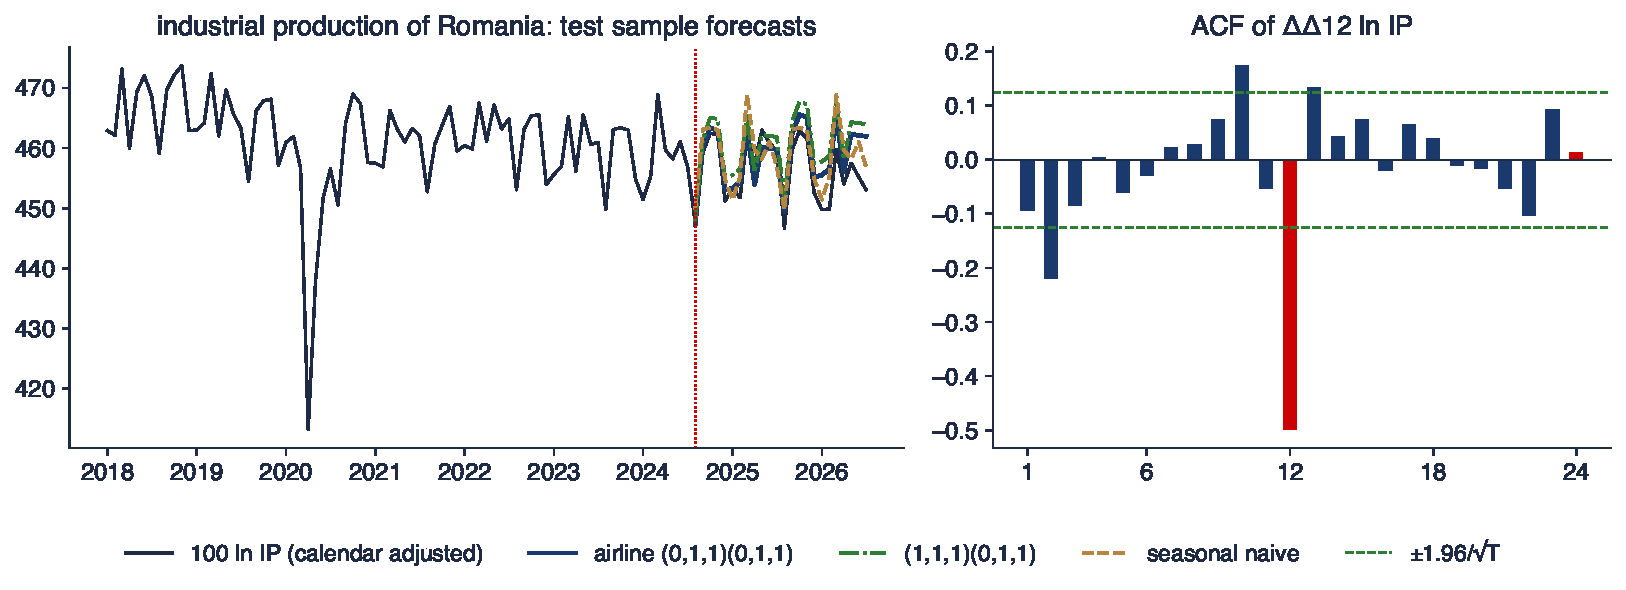
\includegraphics[width=0.96\textwidth,height=0.36\textheight,keepaspectratio]{ch15_sem_b1.pdf}
\end{center}
\vspace{-2mm}
\begin{center}
\scriptsize
\begin{tabular}{lccccc}
\toprule
\textbf{Model} & AICc & BIC & LB(12) $p$ & LB(24) $p$ & test RMSE \\
\midrule
airline $(0,1,1)(0,1,1)_{12}$ & 1304.2 & 1314.3 & 0.065 & 0.432 & 3.75 \\
$(1,1,1)(0,1,1)_{12}$ & 1291.1 & 1304.5 & 0.789 & 0.972 & 5.29 \\
seasonal naive & & & & & 3.85 \\
\bottomrule
\end{tabular}
\end{center}
\begin{itemize}
    \item Tests: ADF $\tau = \ensuremath{-}1.31$ ($p = 0.885$) and KPSS 0.523 $>$ 0.146 for the level; $z_t$: ADF $\ensuremath{-}6.47$, KPSS 0.055: $d = D = 1$; ACF of $z_t$: $\ensuremath{-}0.09$, $\ensuremath{-}0.22$ at lags 1, 2, $\ensuremath{-}0.50$ at 12
    \item Airline: $\hat\theta = \ensuremath{-}0.205$, $\hat\Theta = \ensuremath{-}0.934$; the $(1,1,1)$ model: $\hat\phi = 0.574$, $\hat\theta = \ensuremath{-}0.828$, almost cancelling factors
    \item Interpretation: the $(1,1,1)$ model wins in sample (BIC, clean residuals) but loses out of sample; the airline model is slightly better than the seasonal naive method: use the airline model, and keep the seasonal naive method as the benchmark
\end{itemize}\quantlet{TSA\_ch15\_seminar}{\qlurl{TSA_ch15_seminar}}
\end{frame}

\begin{frame}{B2: volatility of the BET since 2015 [Proposed]}
\itemsize{\footnotesize}
\begin{itemize}
\item \textbf{Question}: is the Bucharest market calmer or more turbulent today than usual, and what does it mean for tomorrow's VaR 1\%? Model: Seminar 5, B1.
\item \textbf{Inputs}: BET daily log returns in \%, January 2015 -- September 2026 ($n = 2\,925$)
\item \textbf{Tasks}
\begin{enumerate}
    \item Run the ARCH-LM test with five lags on the demeaned returns.
    \item Fit a GARCH(1,1) with Student-$t$ innovations; report the persistence and the half-life.
    \item Compare the long-run, the sample and today's annualised volatility.
    \item Compute tomorrow's VaR 1\% with the $t$ and with the Normal quantile.
    \item Interpretation: is the BET calmer or more turbulent than usual today?
\end{enumerate}
\item \textbf{Report}: one test, five parameters, three volatilities, two VaR values and one sentence
\item Notebook: section B2
\end{itemize}
\end{frame}

\ifsolutions
\begin{frame}{B2: solution [Proposed]}
\itemsize{\footnotesize}
\begin{itemize}
    \item ARCH-LM(5) $= 366.8$, $p$ $<$\,0.001: strong ARCH effects
    \item GARCH(1,1)-$t$: $\mu = 0.087$, $\omega = 0.069$, $\alpha = 0.185$, $\beta = 0.740$, $\nu = 5.01$; persistence 0.925, half-life 8.8 days
    \item Volatility: long run 15.1\%, sample 15.5\%, today 25.5\% a year
    \item VaR 1\% for tomorrow: 4.11\% with the $t$ quantile, 3.66\% with the Normal one
    \item Interpretation: today the BET is more turbulent than usual (25.5\% against 15.1\%); with a half-life of about 8.8 days the excess fades within weeks; until then the VaR is higher than its average level
\end{itemize}\quantlet{TSA\_ch15\_seminar}{\qlurl{TSA_ch15_seminar}}
\end{frame}
\fi

\begin{frame}{B3: the Romanian and German 10-year yields [Proposed]}
\itemsize{\footnotesize}
\begin{itemize}
\item \textbf{Question}: is the Romanian 10-year yield tied to the German one in the long run? Model: Seminar 7, B1 and A3.
\item \textbf{Inputs}: monthly means of daily 10-year yields (\%), January 2008 -- September 2026 ($T = 224$)
\item \textbf{Tasks}
\begin{enumerate}
    \item Run ADF on both yields and on their differences.
    \item Run the Engle--Granger test (Romania on Germany) and report $\hat\beta$.
    \item Run the Johansen trace and maximum-eigenvalue tests.
    \item Estimate the error-correction equation of each yield and compute the half-life.
    \item Interpretation: is the Romanian yield tied to the German one?
\end{enumerate}
\item \textbf{Report}: four ADF results, two cointegration tests, two adjustment coefficients and one sentence
\item Notebook: section B3
\end{itemize}
\end{frame}

\ifsolutions
\begin{frame}{B3: solution [Proposed]}
\itemsize{\scriptsize}
\begin{itemize}
    \item ADF: levels $\ensuremath{-}2.25$ ($p = 0.189$) and $\ensuremath{-}1.97$ ($p = 0.298$): $I(1)$; differences $\ensuremath{-}4.08$ and $\ensuremath{-}6.38$: stationary
    \item Engle--Granger: $\tau = \ensuremath{-}4.23 < \ensuremath{-}3.36$ ($p = 0.003$): cointegrated; $\hat y^{RO} = 3.92 + 1.35\,y^{DE}$
    \item Johansen: trace 15.87 $>$ 15.49 ($r = 0$ rejected, at the border), 2.03 $<$ 3.84; maximum eigenvalue 13.84 $<$ 14.26: not rejected
    \item ECM: Romania $\gamma = \ensuremath{-}0.036$ ($t = \ensuremath{-}1.87$), half-life 19 months; Germany $\gamma = 0.021$ ($t = 2.00$); short run $\Delta y^{RO}$ on $\Delta y^{DE}$: 0.284 ($t = 2.29$)
    \item Interpretation: a weak and slow long-run link: the spread (mean 4.45 pp) returns to equilibrium in years, $\hat\beta > 1$ means Romanian yields move more than German ones; the evidence depends on the test, so the honest answer is ``probably, but weakly''
\end{itemize}\quantlet{TSA\_ch15\_seminar}{\qlurl{TSA_ch15_seminar}}
\end{frame}
\fi


%=============================================================================
\section{Part C: an open idea and AI critique}
%=============================================================================

\begin{frame}{C1: a forecast competition for Romanian inflation [Proposed]}
\itemsize{\footnotesize}
\begin{itemize}
\item \textbf{Question}: which method would have forecast Romanian monthly inflation best over the last ten years, one and twelve months ahead?
\item \textbf{Inputs}: the Romanian HICP (Eurostat), monthly, 2005--2026; Lecture 15 runs one SARIMA on one test sample
\item \textbf{Tasks}
\begin{enumerate}
    \item List five competitors: seasonal naive, SES, SARIMA, ARFIMA, a ridge model with lags and month dummies.
    \item Describe a rolling-origin design: first origin, step, horizons, refits.
    \item Say how you would treat the tax changes of 2010, 2015 and 2025.
    \item Choose the error measures and the test for the comparison.
\end{enumerate}
\item \textbf{Report}: a one-page plan that a team could turn into its project
\item Notebook: section C1
\end{itemize}
\end{frame}

\ifsolutions
\begin{frame}{C1: a reference plan [Proposed]}
\itemsize{\footnotesize}
\begin{itemize}
    \item Origins every month from January 2015; horizons 1 and 12; every model refitted at every origin, orders chosen on data before the origin
    \item Tax changes: dummies known in advance (VAT dates are announced) or a robust loss; report results with and without the tax months
    \item MASE against the seasonal naive method; Diebold--Mariano with the HLN correction for each pair; a table by horizon
    \item Expected result: small gains at one month, almost none at twelve months; ARFIMA and SARIMA close; a combination hard to beat
\end{itemize}
\end{frame}
\fi

\begin{frame}{C2: audit an AI answer [Proposed]}
\itemsize{\scriptsize}
\begin{itemize}
    \item A student asked an AI assistant to check the answers to Part A. The answer:
    \item \aiprompt{(a) For the unemployment rate, ADF gives p = 0.52, so the unit root is rejected at 5\%.}
    \item \aiprompt{(b) KPSS = 1.04 > 0.463 rejects, so the level of unemployment is stationary.}
    \item \aiprompt{(c) For the DAX, alpha + beta = 0.992, so a shock halves in 1/(1 - 0.992) = 128 days.}
    \item \aiprompt{(d) The VaR 99\% of the DAX for tomorrow is -2.31\%.}
    \item \aiprompt{(e) Inflation Granger-causes ROBOR (p = 0.036), which proves that inflation causes the central bank to raise rates.}
    \item \aiprompt{(f) Ljung-Box Q(12) on the residuals of an AR(1) x SAR(1) model has 12 degrees of freedom.}
    \item Tasks
    \begin{itemize}
        \item 1. For each statement, say whether it is correct; if not, give the correct statement and the correct number (notebook, section C2).
        \item 2. Report: six verdicts with one line of justification each.
    \end{itemize}
\end{itemize}
\end{frame}

\ifsolutions
\begin{frame}{C2: solution [Proposed]}
\itemsize{\footnotesize}
\begin{itemize}
    \item (a) Wrong: $p = 0.52 > 0.05$: the unit root is not rejected; $u_t \sim I(1)$
    \item (b) Wrong: $H_0$ of KPSS is stationarity; rejecting it points to a unit root
    \item (c) Wrong: $h_{1/2} = \ln 0.5/\ln 0.992 = 88$ days; $1/(1 - \alpha - \beta)$ is not a half-life
    \item (d) Wrong twice: the level is the tail probability, VaR 1\%, and VaR is a positive loss: 2.31\%
    \item (e) Wrong: Granger causality is extra predictability, not proof of a causal policy effect
    \item (f) Wrong: $12 - 2 = 10$ degrees of freedom (two estimated ARMA parameters)
\end{itemize}\quantlet{TSA\_ch15\_seminar}{\qlurl{TSA_ch15_seminar}}
\end{frame}
\fi


%=============================================================================
\section{Wrap-up}
%=============================================================================

\begin{frame}{Key takeaways}
\itemsize{\small}
\begin{itemize}
    \item Every exam problem has three parts: the formula with the numbers, the result with its unit and sign, the interpretation
    \item Tests: state $H_0$ first; ADF and KPSS have opposite nulls; Ljung--Box on residuals loses $k$ degrees of freedom
    \item Forecasts by hand: write the model in levels of $z_t$, substitute the last values, then undo the differences
    \item A better in-sample model is not a better forecaster (B1); judge it on a test sample against a benchmark
    \item An AI answer is a draft: check the null hypotheses, the half-life, the VaR level and the degrees of freedom
\end{itemize}
\end{frame}

\begin{frame}{After the seminar}
\itemsize{\small}
\begin{itemize}
    \item Lecture 15 gathers the course: the course map, one recap slide per chapter, the toolbox, Box--Jenkins on Romanian inflation, eight solved exam-type problems, the project
    \item Try the [Proposed] tasks on paper first, then check them in the notebook
    \item C1 can grow into a team project
    \item Reading: \refHP; \refFPP; \refBJ
    \item \textbf{The seminar is for practice and is not graded; the solutions of [Proposed] tasks are discussed in class}
\end{itemize}
\end{frame}


%=============================================================================
\section{References}
%=============================================================================

\begin{frame}{References}
\itemsize{\tiny}
\begin{itemize}
    \item Bollerslev, T. (1986). Generalized autoregressive conditional heteroskedasticity. \textit{Journal of Econometrics}, 31(3), 307--327. \href{https://doi.org/10.1016/0304-4076(86)90063-1}{doi:10.1016/0304-4076(86)90063-1}
    \item Box, G. E. P., Jenkins, G. M., \& Reinsel, G. C. (2008). \textit{Time Series Analysis: Forecasting and Control} (4th ed.). Wiley. \href{https://doi.org/10.1002/9781118619193}{doi:10.1002/9781118619193}
    \item Dickey, D. A., \& Fuller, W. A. (1979). Distribution of the estimators for autoregressive time series with a unit root. \textit{Journal of the American Statistical Association}, 74(366), 427--431. \href{https://doi.org/10.1080/01621459.1979.10482531}{doi:10.1080/01621459.1979.10482531}
    \item Diebold, F. X., \& Mariano, R. S. (1995). Comparing predictive accuracy. \textit{Journal of Business \& Economic Statistics}, 13(3), 253--263. \href{https://doi.org/10.1080/07350015.1995.10524599}{doi:10.1080/07350015.1995.10524599}
    \item Engle, R. F., \& Granger, C. W. J. (1987). Co-integration and error correction: Representation, estimation, and testing. \textit{Econometrica}, 55(2), 251--276. \href{https://doi.org/10.2307/1913236}{doi:10.2307/1913236}
    \item Granger, C. W. J. (1969). Investigating causal relations by econometric models and cross-spectral methods. \textit{Econometrica}, 37(3), 424--438. \href{https://doi.org/10.2307/1912791}{doi:10.2307/1912791}
    \item Huang, C., \& Petukhina, A. (2022). \textit{Applied Time Series Analysis and Forecasting with Python}. Springer. \href{https://doi.org/10.1007/978-3-031-13584-2}{doi:10.1007/978-3-031-13584-2}
    \item Hyndman, R. J., \& Athanasopoulos, G. (2021). \textit{Forecasting: Principles and Practice} (3rd ed.). OTexts. \href{https://otexts.com/fpp3/}{otexts.com/fpp3}
    \item Johansen, S. (1991). Estimation and hypothesis testing of cointegration vectors in Gaussian vector autoregressive models. \textit{Econometrica}, 59(6), 1551--1580. \href{https://doi.org/10.2307/2938278}{doi:10.2307/2938278}
    \item Kwiatkowski, D., Phillips, P. C. B., Schmidt, P., \& Shin, Y. (1992). Testing the null hypothesis of stationarity against the alternative of a unit root. \textit{Journal of Econometrics}, 54(1--3), 159--178. \href{https://doi.org/10.1016/0304-4076(92)90104-Y}{doi:10.1016/0304-4076(92)90104-Y}
    \item Ljung, G. M., \& Box, G. E. P. (1978). On a measure of lack of fit in time series models. \textit{Biometrika}, 65(2), 297--303. \href{https://doi.org/10.1093/biomet/65.2.297}{doi:10.1093/biomet/65.2.297}
\end{itemize}
\end{frame}

\end{document}
